% =====================================================================
%  libreta.tex
%  ========================
%
%
%  Descripción:
%  ------------
%  Apuntes de clase del curso de Fundamentos para el Análisis 
%  Automático de Lenguaje.
%
%
%  Metadata:
%  ----------
%   * Author : zxxz6 (Bryan Violante Arriaga)
%   * Version: 2.9.0
%
%
%  History:
%  ------------
%  Author      Date            Description
%  zxxz6       25/09/2026      Clase 23 Sep, TCOR, random indexing y LSI
%  zxxz6       21/09/2026      Clase 21 Sep, WSD e indexado conceptual
%  zxxz6       14/09/2026      Clase 14 Sep, indexado mas alla de la palabra
%  zxxz6       09/09/2026      Clase 9 Sep, representaciones y POS tagging
%  zxxz6       09/09/2026      Nombre el algoritmo de Porter en preprocesado
%  zxxz6       09/09/2026      Clase 7 Sep, expansion de consultas y clustering
%  zxxz6       31/08/2026      Clase 31 Ago, modelos de lenguaje y evaluacion
%  zxxz6       26/08/2026      Clase 26 Ago, continuacion del VSM
%  zxxz6       24/08/2026      Clase 24 Ago, IR
%  zxxz6       19/08/2026      Apuntes de la clase del 19 de agosto
%  zxxz6       19/08/2026      Registre a los cuatro profesores
%  zxxz6       17/08/2026      Creation
%
%
% =====================================================================
\documentclass[11pt,letterpaper]{article}

% =====================================================================
%  DATOS DE LA MATERIA
% =====================================================================
\newcommand{\materia}{Fundamentos para el Análisis Automático de Lenguaje}
\newcommand{\profesor}{Dra. Delia Irazú Hernández Farías \\
                       Dr. Luis Villaseñor Pineda \\
                       Dr. Manuel Montes y Gómez \\
                       Dr. Aurelio López López}
\newcommand{\periodo}{Otoño 2026}
\newcommand{\alumno}{Bryan Ezequiel Violante Arriaga}

% =====================================================================
%  Preambulo.tex
%  ========================
%
%
%  Descripción:
%  ------------
%  Preámbulo compartido de los apuntes de clase: paquetes, estilo de
%  página, entornos de teorema, las cuatro cajas de color, el estilo de
%  listings y el pseudocódigo en español. Se carga con \input desde
%  cada documento en lugar de copiarlo, para que un arreglo aquí llegue
%  a todas las libretas de una vez.
%
%
%  Considerations:
%  ------------
%  - Se carga con \input y ruta relativa, no con \usepackage, porque
%    \usepackage solo busca en la carpeta del documento y en el árbol
%    de TeX. Un .sty instalado en TEXMFHOME evitaría la ruta, pero vive
%    fuera del repo y una clona nueva no compilaría
%  - Los cuatro datos de la materia se declaran en el documento ANTES
%    del \input. hyperref expande \materia al cargarse, así que si no
%    existe todavía la compilación truena
%  - Cuando la materia la imparte más de un profesor, los nombres van
%    en un solo \profesor separados por \\. La portadilla los imprime
%    dentro de un center, que es donde \\ sí corta renglón. Repetir
%    \newcommand{\profesor} no es opción: truena con "already defined"
%  - algorithmicx no tiene opción de idioma y babel no lo traduce, así
%    que las palabras clave del pseudocódigo se renombran a mano
%  - Los nombres de los entornos van sin acento (\begin{definicion})
%    aunque el rótulo impreso sí lo lleve
%  - babel se carga con es-noshorthands porque en español el " queda
%    activo y se come el texto que le sigue, además de romper listings
%
%
%  Metadata:
%  ----------
%   * Author : zxxz6 (Bryan Violante Arriaga)
%   * Version: 1.7.0
%
%
%  History:
%  ------------
%  Author      Date            Description
%  zxxz6       24/09/2026      El nombre del alumno en el encabezado
%  zxxz6       24/09/2026      Encabezado de una hoja de un ejercicio
%  zxxz6       23/09/2026      Macros de los documentos de soluciones
%  zxxz6       30/08/2026      Macros de lim, limsup y liminf sobre n
%  zxxz6       25/08/2026      Macros de Omega, Theta, o y omega chicas
%  zxxz6       20/08/2026      Cargue pgfplots para graficas de datos
%  zxxz6       20/08/2026      Cargue tikz para diagramas de conjuntos
%  zxxz6       19/08/2026      Documente \profesor con varios nombres
%  zxxz6       19/08/2026      Agregue la caja Idea Random
%  zxxz6       18/08/2026      Creation
%
%
% =====================================================================
%  USO
%  ---
%  \documentclass[11pt,letterpaper]{article}
%  \newcommand{\materia}{...}      % los cuatro datos van arriba
%  \newcommand{\profesor}{...}
%  \newcommand{\periodo}{...}
%  \newcommand{\alumno}{...}
%  % =====================================================================
%  Preambulo.tex
%  ========================
%
%
%  Descripción:
%  ------------
%  Preámbulo compartido de los apuntes de clase: paquetes, estilo de
%  página, entornos de teorema, las cuatro cajas de color, el estilo de
%  listings y el pseudocódigo en español. Se carga con \input desde
%  cada documento en lugar de copiarlo, para que un arreglo aquí llegue
%  a todas las libretas de una vez.
%
%
%  Considerations:
%  ------------
%  - Se carga con \input y ruta relativa, no con \usepackage, porque
%    \usepackage solo busca en la carpeta del documento y en el árbol
%    de TeX. Un .sty instalado en TEXMFHOME evitaría la ruta, pero vive
%    fuera del repo y una clona nueva no compilaría
%  - Los cuatro datos de la materia se declaran en el documento ANTES
%    del \input. hyperref expande \materia al cargarse, así que si no
%    existe todavía la compilación truena
%  - Cuando la materia la imparte más de un profesor, los nombres van
%    en un solo \profesor separados por \\. La portadilla los imprime
%    dentro de un center, que es donde \\ sí corta renglón. Repetir
%    \newcommand{\profesor} no es opción: truena con "already defined"
%  - algorithmicx no tiene opción de idioma y babel no lo traduce, así
%    que las palabras clave del pseudocódigo se renombran a mano
%  - Los nombres de los entornos van sin acento (\begin{definicion})
%    aunque el rótulo impreso sí lo lleve
%  - babel se carga con es-noshorthands porque en español el " queda
%    activo y se come el texto que le sigue, además de romper listings
%
%
%  Metadata:
%  ----------
%   * Author : zxxz6 (Bryan Violante Arriaga)
%   * Version: 1.7.0
%
%
%  History:
%  ------------
%  Author      Date            Description
%  zxxz6       24/09/2026      El nombre del alumno en el encabezado
%  zxxz6       24/09/2026      Encabezado de una hoja de un ejercicio
%  zxxz6       23/09/2026      Macros de los documentos de soluciones
%  zxxz6       30/08/2026      Macros de lim, limsup y liminf sobre n
%  zxxz6       25/08/2026      Macros de Omega, Theta, o y omega chicas
%  zxxz6       20/08/2026      Cargue pgfplots para graficas de datos
%  zxxz6       20/08/2026      Cargue tikz para diagramas de conjuntos
%  zxxz6       19/08/2026      Documente \profesor con varios nombres
%  zxxz6       19/08/2026      Agregue la caja Idea Random
%  zxxz6       18/08/2026      Creation
%
%
% =====================================================================
%  USO
%  ---
%  \documentclass[11pt,letterpaper]{article}
%  \newcommand{\materia}{...}      % los cuatro datos van arriba
%  \newcommand{\profesor}{...}
%  \newcommand{\periodo}{...}
%  \newcommand{\alumno}{...}
%  % =====================================================================
%  Preambulo.tex
%  ========================
%
%
%  Descripción:
%  ------------
%  Preámbulo compartido de los apuntes de clase: paquetes, estilo de
%  página, entornos de teorema, las cuatro cajas de color, el estilo de
%  listings y el pseudocódigo en español. Se carga con \input desde
%  cada documento en lugar de copiarlo, para que un arreglo aquí llegue
%  a todas las libretas de una vez.
%
%
%  Considerations:
%  ------------
%  - Se carga con \input y ruta relativa, no con \usepackage, porque
%    \usepackage solo busca en la carpeta del documento y en el árbol
%    de TeX. Un .sty instalado en TEXMFHOME evitaría la ruta, pero vive
%    fuera del repo y una clona nueva no compilaría
%  - Los cuatro datos de la materia se declaran en el documento ANTES
%    del \input. hyperref expande \materia al cargarse, así que si no
%    existe todavía la compilación truena
%  - Cuando la materia la imparte más de un profesor, los nombres van
%    en un solo \profesor separados por \\. La portadilla los imprime
%    dentro de un center, que es donde \\ sí corta renglón. Repetir
%    \newcommand{\profesor} no es opción: truena con "already defined"
%  - algorithmicx no tiene opción de idioma y babel no lo traduce, así
%    que las palabras clave del pseudocódigo se renombran a mano
%  - Los nombres de los entornos van sin acento (\begin{definicion})
%    aunque el rótulo impreso sí lo lleve
%  - babel se carga con es-noshorthands porque en español el " queda
%    activo y se come el texto que le sigue, además de romper listings
%
%
%  Metadata:
%  ----------
%   * Author : zxxz6 (Bryan Violante Arriaga)
%   * Version: 1.7.0
%
%
%  History:
%  ------------
%  Author      Date            Description
%  zxxz6       24/09/2026      El nombre del alumno en el encabezado
%  zxxz6       24/09/2026      Encabezado de una hoja de un ejercicio
%  zxxz6       23/09/2026      Macros de los documentos de soluciones
%  zxxz6       30/08/2026      Macros de lim, limsup y liminf sobre n
%  zxxz6       25/08/2026      Macros de Omega, Theta, o y omega chicas
%  zxxz6       20/08/2026      Cargue pgfplots para graficas de datos
%  zxxz6       20/08/2026      Cargue tikz para diagramas de conjuntos
%  zxxz6       19/08/2026      Documente \profesor con varios nombres
%  zxxz6       19/08/2026      Agregue la caja Idea Random
%  zxxz6       18/08/2026      Creation
%
%
% =====================================================================
%  USO
%  ---
%  \documentclass[11pt,letterpaper]{article}
%  \newcommand{\materia}{...}      % los cuatro datos van arriba
%  \newcommand{\profesor}{...}
%  \newcommand{\periodo}{...}
%  \newcommand{\alumno}{...}
%  \input{../../templates/Preambulo.tex}
%  \begin{document}
%  \portadilla
%
%  Con dos o mas profesores se declara UN solo \profesor y los nombres
%  se separan con \\, uno por renglon:
%
%  \newcommand{\profesor}{Dra. Fulana de Tal \\
%                         Dr. Mengano de Cual}
% =====================================================================


% ==================== IDIOMA Y CODIFICACIÓN ====================
\usepackage[utf8]{inputenc}
\usepackage[T1]{fontenc}
\usepackage[spanish,es-tabla,es-noshorthands]{babel}
\usepackage{lmodern}
\usepackage{microtype}

% ==================== PÁGINA ====================
\usepackage[letterpaper,margin=2.3cm,headheight=14pt]{geometry}
\usepackage{parskip}
\usepackage{fancyhdr}
\usepackage{enumitem}

% ==================== MATEMÁTICAS ====================
\usepackage{amsmath,amssymb,amsthm,mathtools}

% ==================== FIGURAS, TABLAS, CÓDIGO ====================
\usepackage{graphicx}
\usepackage{booktabs}
\usepackage{array}
% float da el especificador [H], que clava una tabla donde se
% escribio. Una traza que LaTeX manda dos paginas adelante deja
% de leerse junto al paso que la produjo
\usepackage{float}
\usepackage{xcolor}
% tikz ya viene arrastrado por tcolorbox[most], pero se carga
% explicito para no depender de ese detalle; la libreria babel
% protege a tikz de los caracteres activos del español
\usepackage{tikz}
\usetikzlibrary{babel}
% pgfplots dibuja graficas de datos (ejes, escalas log) sobre tikz
\usepackage{pgfplots}
\pgfplotsset{compat=1.18}
\usepackage{listings}
\usepackage[ruled,section]{algorithm}
\usepackage{algpseudocode}
\usepackage[most]{tcolorbox}
% soul da \hl, el unico resaltado que parte renglon; \colorbox no
\usepackage{soul}
\usepackage{hyperref}

% =====================================================================
%  ESTILO
% =====================================================================

% --- encabezado y pie de cada página ---
\pagestyle{fancy}
\fancyhf{}
\fancyhead[L]{\small\textsc{\materia}}
\fancyhead[R]{\small\periodo}
\fancyfoot[C]{\small\thepage}
\renewcommand{\headrulewidth}{0.4pt}

% --- enlaces ---
\hypersetup{
  colorlinks=true,
  linkcolor=black,
  urlcolor=blue,
  citecolor=black,
  pdftitle={Apuntes de \materia},
  pdfauthor={\alumno}
}

% --- paleta ---
\definecolor{acento}{HTML}{1F4E79}
\definecolor{fondoIdea}{HTML}{EAF2FB}
\definecolor{fondoOjo}{HTML}{FDF0E6}
\definecolor{fondoPend}{HTML}{F2F0F7}
\definecolor{comentario}{HTML}{5A7D5A}
\definecolor{cadena}{HTML}{A03030}
\definecolor{fondoCodigo}{HTML}{F7F7F7}
\definecolor{fondoResultado}{HTML}{EAF5EC}
\definecolor{marcador}{HTML}{FFF3A3}

% --- entornos de teorema; numeran por sección, o sea por clase ---
\theoremstyle{definition}
\newtheorem{definicion}{Definición}[section]
\newtheorem{ejemplo}[definicion]{Ejemplo}
\newtheorem{ejercicio}[definicion]{Ejercicio}

\theoremstyle{plain}
\newtheorem{teorema}[definicion]{Teorema}
\newtheorem{lema}[definicion]{Lema}
\newtheorem{corolario}[definicion]{Corolario}
\newtheorem{proposicion}[definicion]{Proposición}

\theoremstyle{remark}
\newtheorem*{observacion}{Observación}
\newtheorem*{quick_sum}{Resumen rápido}

% --- cajas de color para lo que se relee antes del examen ---
\newtcolorbox{idea}[1][]{
  colback=fondoIdea, colframe=acento, boxrule=0.6pt,
  arc=2pt, left=6pt, right=6pt, top=5pt, bottom=5pt,
  title={Idea clave}, fonttitle=\bfseries\small, #1
}
\newtcolorbox{ojo}[1][]{
  colback=fondoOjo, colframe=orange!70!black, boxrule=0.6pt,
  arc=2pt, left=6pt, right=6pt, top=5pt, bottom=5pt,
  title={Ojito...}, fonttitle=\bfseries\small, #1
}
\newtcolorbox{pendiente}[1][]{
  colback=fondoPend, colframe=violet!60!black, boxrule=0.6pt,
  arc=2pt, left=6pt, right=6pt, top=5pt, bottom=5pt,
  title={Pendiente por resolver}, fonttitle=\bfseries\small, #1
}
\newtcolorbox{idear}[1][]{
  colback=fondoPend, colframe=pink!60!black, boxrule=0.6pt,
  arc=2pt, left=6pt, right=6pt, top=5pt, bottom=5pt,
  title={Idea Random}, fonttitle=\bfseries\small, #1
}

% --- el resultado al que llego un ejercicio, para que se vea de
%     lejos al hojear la hoja antes del examen ---
\newtcolorbox{resultado}[1][]{
  colback=fondoResultado, colframe=green!45!black, boxrule=0.6pt,
  arc=2pt, left=6pt, right=6pt, top=5pt, bottom=5pt,
  title={Resultado}, fonttitle=\bfseries\small, #1
}

% --- código ---
\lstdefinestyle{codigo}{
  backgroundcolor=\color{fondoCodigo},
  basicstyle=\ttfamily\footnotesize,
  keywordstyle=\color{acento}\bfseries,
  commentstyle=\color{comentario}\itshape,
  stringstyle=\color{cadena},
  numbers=left, numberstyle=\tiny\color{gray}, numbersep=8pt,
  frame=single, rulecolor=\color{gray!40},
  breaklines=true, showstringspaces=false,
  tabsize=4, captionpos=b,
  extendedchars=true, inputencoding=utf8,
  literate={á}{{\'a}}1 {é}{{\'e}}1 {í}{{\'i}}1
           {ó}{{\'o}}1 {ú}{{\'u}}1 {ñ}{{\~n}}1
           {Ü}{{\"U}}1 {ü}{{\"u}}1 {¿}{{?`}}1
           {¡}{{!`}}1
}
\lstset{style=codigo}
\renewcommand{\lstlistingname}{Código}
\renewcommand{\lstlistlistingname}{Índice de código}
% --- pseudocódigo; algorithmicx arma el cuerpo y algorithm el
%     flotante que lo numera y lo pone en el índice. Las palabras
%     clave vienen en inglés de fábrica y babel no las toca, así que
%     se renombran una por una ---
\floatname{algorithm}{Algoritmo}
\renewcommand{\listalgorithmname}{Índice de algoritmos}

\algrenewcommand\algorithmicrequire{\textbf{Entrada:}}
\algrenewcommand\algorithmicensure{\textbf{Salida:}}
\algrenewcommand\algorithmicend{\textbf{fin}}
\algrenewcommand\algorithmicif{\textbf{si}}
\algrenewcommand\algorithmicthen{\textbf{entonces}}
\algrenewcommand\algorithmicelse{\textbf{si no}}
\algrenewcommand\algorithmicfor{\textbf{para}}
\algrenewcommand\algorithmicforall{\textbf{para todo}}
\algrenewcommand\algorithmicdo{\textbf{hacer}}
\algrenewcommand\algorithmicwhile{\textbf{mientras}}
\algrenewcommand\algorithmicrepeat{\textbf{repetir}}
\algrenewcommand\algorithmicuntil{\textbf{hasta que}}
\algrenewcommand\algorithmicloop{\textbf{ciclo}}
\algrenewcommand\algorithmicprocedure{\textbf{procedimiento}}
\algrenewcommand\algorithmicfunction{\textbf{función}}
\algrenewcommand\algorithmicreturn{\textbf{devolver}}
\algrenewcomment[1]{\hfill{\color{comentario}\itshape // #1}}

% Las dos que algorithmicx no trae. El \ del final es obligatorio: sin
% el TeX se come el espacio y sale "hastan-1" en vez de "hasta n-1"
\algnewcommand\Hasta{\textbf{hasta}\ }
\algnewcommand\Intercambiar{\textbf{intercambiar}\ }

% --- abreviaturas que se usan a cada rato ---
\newcommand{\N}{\mathbb{N}}
\newcommand{\Z}{\mathbb{Z}}
\newcommand{\Q}{\mathbb{Q}}
\newcommand{\R}{\mathbb{R}}
\newcommand{\C}{\mathbb{C}}
\newcommand{\abs}[1]{\left\lvert #1 \right\rvert}
\newcommand{\norm}[1]{\left\lVert #1 \right\rVert}
\newcommand{\set}[1]{\left\{ #1 \right\}}
\newcommand{\Ord}[1]{\mathcal{O}\!\left(#1\right)}
% Mayuscula la notacion grande, minuscula la chica
\newcommand{\Omg}[1]{\Omega\!\left(#1\right)}
\newcommand{\Tht}[1]{\Theta\!\left(#1\right)}
\newcommand{\ord}[1]{o\!\left(#1\right)}
\newcommand{\omg}[1]{\omega\!\left(#1\right)}
% Los tres limites sobre n, que salen en cada renglon del criterio
% del cociente para la notacion asintotica
\newcommand{\LM}{\lim_{n \to \infty}}
\newcommand{\LS}{\limsup_{n \to \infty}}
\newcommand{\LI}{\liminf_{n \to \infty}}

% --- encabezado de cada sesión: título a la izquierda, fecha a la
%     derecha. El argumento corto es el que sale en el índice ---
\newcommand{\clase}[2]{%
  \section[#1]{#1 \hfill \normalfont\small\textit{#2}}%
}

% --- portadilla y tabla de contenidos. Se llama una vez, justo
%     despues de \begin{document}. El renglon del profesor va dentro
%     del center, asi que \profesor puede traer varios nombres
%     separados por \\ y salen apilados y centrados sin tocar nada ---
\newcommand{\portadilla}{%
  \begin{center}
    {\LARGE\bfseries\materia\par}
    \vspace{0.4em}
    {\large \profesor \par}
    \vspace{0.2em}
    {\small \periodo\quad-\quad\alumno\par}
    \vspace{0.3em}
    \rule{\linewidth}{0.5pt}
  \end{center}
  \vspace{0.5em}
  \tableofcontents
  \vspace{1em}
  \rule{\linewidth}{0.5pt}%
}

% =====================================================================
%  DOCUMENTOS DE SOLUCIONES
%  Lo que usa una tanda de ejercicios resueltos. Una libreta no toca
%  nada de aqui, pero vive en el preambulo compartido para no tener
%  dos archivos que arreglar cuando cambie el estilo.
% =====================================================================

% --- encabezado compacto: titulo, subtitulo y regla. Sustituye a
%     \portadilla cuando el documento es una tanda de ejercicios: sin
%     indice, porque se hojea de corrido, no se navega ---
\newcommand{\encabezadoSoluciones}[2]{%
  % El paquete algorithm se carga con la opcion [section] para que en
  % una libreta el pseudocodigo se numere por clase. Aqui no hay
  % secciones, asi que esa numeracion sale como "Algoritmo 0.1". Se
  % corrige al vuelo, y solo en los documentos que llaman a este
  % encabezado: la libreta no se entera.
  \renewcommand{\thealgorithm}{\arabic{algorithm}}%
  \begin{center}
    {\LARGE\bfseries #1\par}
    \vspace{0.3em}
    {\small\itshape #2\par}
    \vspace{0.5em}
    \rule{\linewidth}{0.5pt}
  \end{center}
  \vspace{0.3em}%
}

% --- hoja de un solo ejercicio: un renglon chico arriba con el
%     titulo y su numero, y ya. Sin titulo grande y sin pie de pagina,
%     porque en una hoja de dos paginas cada centimetro que se va en
%     adornos es un paso del desarrollo que no cabe ---
\newcommand{\encabezadoEjercicio}[3]{%
  % Misma correccion que en \encabezadoSoluciones: sin secciones, el
  % pseudocodigo saldria numerado "0.1"
  \renewcommand{\thealgorithm}{\arabic{algorithm}}%
  \fancyhf{}%
  \fancyhead[L]{\small\textsc{#1} (ejercicio #2 de #3)}%
  % El nombre va a la derecha porque las hojas de respuestas se
  % entregan y el profesor pide que cada una lo lleve
  \fancyhead[R]{\small\alumno}%
  \renewcommand{\headrulewidth}{0.4pt}%
  \pagestyle{fancy}%
  \thispagestyle{fancy}%
}

% --- bloque tematico, numerado con romanos: I, II, III. Agrupa los
%     ejercicios que comparten tema. No dibuja regla: la del
%     \problema que sigue ya separa el titulo del primer ejercicio,
%     y dos rayas seguidas dejan un hueco feo ---
\newcounter{parte}
\renewcommand{\theparte}{\Roman{parte}}
\newcommand{\parte}[1]{%
  \bigskip
  \refstepcounter{parte}%
  \noindent{\large\bfseries \theparte. #1\par}%
}

% --- un ejercicio resuelto. Se numera solo y corrido a lo largo del
%     documento, sin reiniciar en cada parte, para poder decir "el 14"
%     sin aclarar de que bloque ---
\newcounter{problema}
\newcommand{\problema}[1]{%
  \bigskip
  \noindent\rule{\linewidth}{0.4pt}\par
  \vspace{0.3em}
  \refstepcounter{problema}%
  \noindent{\bfseries Ejercicio \theproblema\ --- #1\par}
  \vspace{0.3em}%
}

% --- rotulo del paso que sigue: Caso base, Hipotesis inductiva, Paso
%     inductivo. El texto sigue en el mismo renglon ---
\newcommand{\paso}[1]{\par\vspace{0.3em}\noindent\textbf{#1}\ }

% --- la respuesta de un ejercicio, centrada y en un cuadro. El
%     argumento va en modo matematico, sin los delimitadores ---
\newcommand{\respuesta}[1]{%
  \[
    \boxed{\;#1\;}
  \]
}

% --- resaltado inline, como pasarle el plumon a media frase. No
%     admite matematicas adentro: soul rompe con $...$, asi que una
%     formula que hay que destacar va en \respuesta ---
\sethlcolor{marcador}
\newcommand{\resaltar}[1]{\hl{#1}}

% --- justificacion al final de un renglon de \align, en chiquito y
%     entre parentesis, para decir de donde salio el paso ---
\newcommand{\razon}[1]{\quad\text{\small\itshape (#1)}}

%############################ END OF PREAMBULO.TEX #############################
%###############################################################################

%  \begin{document}
%  \portadilla
%
%  Con dos o mas profesores se declara UN solo \profesor y los nombres
%  se separan con \\, uno por renglon:
%
%  \newcommand{\profesor}{Dra. Fulana de Tal \\
%                         Dr. Mengano de Cual}
% =====================================================================


% ==================== IDIOMA Y CODIFICACIÓN ====================
\usepackage[utf8]{inputenc}
\usepackage[T1]{fontenc}
\usepackage[spanish,es-tabla,es-noshorthands]{babel}
\usepackage{lmodern}
\usepackage{microtype}

% ==================== PÁGINA ====================
\usepackage[letterpaper,margin=2.3cm,headheight=14pt]{geometry}
\usepackage{parskip}
\usepackage{fancyhdr}
\usepackage{enumitem}

% ==================== MATEMÁTICAS ====================
\usepackage{amsmath,amssymb,amsthm,mathtools}

% ==================== FIGURAS, TABLAS, CÓDIGO ====================
\usepackage{graphicx}
\usepackage{booktabs}
\usepackage{array}
% float da el especificador [H], que clava una tabla donde se
% escribio. Una traza que LaTeX manda dos paginas adelante deja
% de leerse junto al paso que la produjo
\usepackage{float}
\usepackage{xcolor}
% tikz ya viene arrastrado por tcolorbox[most], pero se carga
% explicito para no depender de ese detalle; la libreria babel
% protege a tikz de los caracteres activos del español
\usepackage{tikz}
\usetikzlibrary{babel}
% pgfplots dibuja graficas de datos (ejes, escalas log) sobre tikz
\usepackage{pgfplots}
\pgfplotsset{compat=1.18}
\usepackage{listings}
\usepackage[ruled,section]{algorithm}
\usepackage{algpseudocode}
\usepackage[most]{tcolorbox}
% soul da \hl, el unico resaltado que parte renglon; \colorbox no
\usepackage{soul}
\usepackage{hyperref}

% =====================================================================
%  ESTILO
% =====================================================================

% --- encabezado y pie de cada página ---
\pagestyle{fancy}
\fancyhf{}
\fancyhead[L]{\small\textsc{\materia}}
\fancyhead[R]{\small\periodo}
\fancyfoot[C]{\small\thepage}
\renewcommand{\headrulewidth}{0.4pt}

% --- enlaces ---
\hypersetup{
  colorlinks=true,
  linkcolor=black,
  urlcolor=blue,
  citecolor=black,
  pdftitle={Apuntes de \materia},
  pdfauthor={\alumno}
}

% --- paleta ---
\definecolor{acento}{HTML}{1F4E79}
\definecolor{fondoIdea}{HTML}{EAF2FB}
\definecolor{fondoOjo}{HTML}{FDF0E6}
\definecolor{fondoPend}{HTML}{F2F0F7}
\definecolor{comentario}{HTML}{5A7D5A}
\definecolor{cadena}{HTML}{A03030}
\definecolor{fondoCodigo}{HTML}{F7F7F7}
\definecolor{fondoResultado}{HTML}{EAF5EC}
\definecolor{marcador}{HTML}{FFF3A3}

% --- entornos de teorema; numeran por sección, o sea por clase ---
\theoremstyle{definition}
\newtheorem{definicion}{Definición}[section]
\newtheorem{ejemplo}[definicion]{Ejemplo}
\newtheorem{ejercicio}[definicion]{Ejercicio}

\theoremstyle{plain}
\newtheorem{teorema}[definicion]{Teorema}
\newtheorem{lema}[definicion]{Lema}
\newtheorem{corolario}[definicion]{Corolario}
\newtheorem{proposicion}[definicion]{Proposición}

\theoremstyle{remark}
\newtheorem*{observacion}{Observación}
\newtheorem*{quick_sum}{Resumen rápido}

% --- cajas de color para lo que se relee antes del examen ---
\newtcolorbox{idea}[1][]{
  colback=fondoIdea, colframe=acento, boxrule=0.6pt,
  arc=2pt, left=6pt, right=6pt, top=5pt, bottom=5pt,
  title={Idea clave}, fonttitle=\bfseries\small, #1
}
\newtcolorbox{ojo}[1][]{
  colback=fondoOjo, colframe=orange!70!black, boxrule=0.6pt,
  arc=2pt, left=6pt, right=6pt, top=5pt, bottom=5pt,
  title={Ojito...}, fonttitle=\bfseries\small, #1
}
\newtcolorbox{pendiente}[1][]{
  colback=fondoPend, colframe=violet!60!black, boxrule=0.6pt,
  arc=2pt, left=6pt, right=6pt, top=5pt, bottom=5pt,
  title={Pendiente por resolver}, fonttitle=\bfseries\small, #1
}
\newtcolorbox{idear}[1][]{
  colback=fondoPend, colframe=pink!60!black, boxrule=0.6pt,
  arc=2pt, left=6pt, right=6pt, top=5pt, bottom=5pt,
  title={Idea Random}, fonttitle=\bfseries\small, #1
}

% --- el resultado al que llego un ejercicio, para que se vea de
%     lejos al hojear la hoja antes del examen ---
\newtcolorbox{resultado}[1][]{
  colback=fondoResultado, colframe=green!45!black, boxrule=0.6pt,
  arc=2pt, left=6pt, right=6pt, top=5pt, bottom=5pt,
  title={Resultado}, fonttitle=\bfseries\small, #1
}

% --- código ---
\lstdefinestyle{codigo}{
  backgroundcolor=\color{fondoCodigo},
  basicstyle=\ttfamily\footnotesize,
  keywordstyle=\color{acento}\bfseries,
  commentstyle=\color{comentario}\itshape,
  stringstyle=\color{cadena},
  numbers=left, numberstyle=\tiny\color{gray}, numbersep=8pt,
  frame=single, rulecolor=\color{gray!40},
  breaklines=true, showstringspaces=false,
  tabsize=4, captionpos=b,
  extendedchars=true, inputencoding=utf8,
  literate={á}{{\'a}}1 {é}{{\'e}}1 {í}{{\'i}}1
           {ó}{{\'o}}1 {ú}{{\'u}}1 {ñ}{{\~n}}1
           {Ü}{{\"U}}1 {ü}{{\"u}}1 {¿}{{?`}}1
           {¡}{{!`}}1
}
\lstset{style=codigo}
\renewcommand{\lstlistingname}{Código}
\renewcommand{\lstlistlistingname}{Índice de código}
% --- pseudocódigo; algorithmicx arma el cuerpo y algorithm el
%     flotante que lo numera y lo pone en el índice. Las palabras
%     clave vienen en inglés de fábrica y babel no las toca, así que
%     se renombran una por una ---
\floatname{algorithm}{Algoritmo}
\renewcommand{\listalgorithmname}{Índice de algoritmos}

\algrenewcommand\algorithmicrequire{\textbf{Entrada:}}
\algrenewcommand\algorithmicensure{\textbf{Salida:}}
\algrenewcommand\algorithmicend{\textbf{fin}}
\algrenewcommand\algorithmicif{\textbf{si}}
\algrenewcommand\algorithmicthen{\textbf{entonces}}
\algrenewcommand\algorithmicelse{\textbf{si no}}
\algrenewcommand\algorithmicfor{\textbf{para}}
\algrenewcommand\algorithmicforall{\textbf{para todo}}
\algrenewcommand\algorithmicdo{\textbf{hacer}}
\algrenewcommand\algorithmicwhile{\textbf{mientras}}
\algrenewcommand\algorithmicrepeat{\textbf{repetir}}
\algrenewcommand\algorithmicuntil{\textbf{hasta que}}
\algrenewcommand\algorithmicloop{\textbf{ciclo}}
\algrenewcommand\algorithmicprocedure{\textbf{procedimiento}}
\algrenewcommand\algorithmicfunction{\textbf{función}}
\algrenewcommand\algorithmicreturn{\textbf{devolver}}
\algrenewcomment[1]{\hfill{\color{comentario}\itshape // #1}}

% Las dos que algorithmicx no trae. El \ del final es obligatorio: sin
% el TeX se come el espacio y sale "hastan-1" en vez de "hasta n-1"
\algnewcommand\Hasta{\textbf{hasta}\ }
\algnewcommand\Intercambiar{\textbf{intercambiar}\ }

% --- abreviaturas que se usan a cada rato ---
\newcommand{\N}{\mathbb{N}}
\newcommand{\Z}{\mathbb{Z}}
\newcommand{\Q}{\mathbb{Q}}
\newcommand{\R}{\mathbb{R}}
\newcommand{\C}{\mathbb{C}}
\newcommand{\abs}[1]{\left\lvert #1 \right\rvert}
\newcommand{\norm}[1]{\left\lVert #1 \right\rVert}
\newcommand{\set}[1]{\left\{ #1 \right\}}
\newcommand{\Ord}[1]{\mathcal{O}\!\left(#1\right)}
% Mayuscula la notacion grande, minuscula la chica
\newcommand{\Omg}[1]{\Omega\!\left(#1\right)}
\newcommand{\Tht}[1]{\Theta\!\left(#1\right)}
\newcommand{\ord}[1]{o\!\left(#1\right)}
\newcommand{\omg}[1]{\omega\!\left(#1\right)}
% Los tres limites sobre n, que salen en cada renglon del criterio
% del cociente para la notacion asintotica
\newcommand{\LM}{\lim_{n \to \infty}}
\newcommand{\LS}{\limsup_{n \to \infty}}
\newcommand{\LI}{\liminf_{n \to \infty}}

% --- encabezado de cada sesión: título a la izquierda, fecha a la
%     derecha. El argumento corto es el que sale en el índice ---
\newcommand{\clase}[2]{%
  \section[#1]{#1 \hfill \normalfont\small\textit{#2}}%
}

% --- portadilla y tabla de contenidos. Se llama una vez, justo
%     despues de \begin{document}. El renglon del profesor va dentro
%     del center, asi que \profesor puede traer varios nombres
%     separados por \\ y salen apilados y centrados sin tocar nada ---
\newcommand{\portadilla}{%
  \begin{center}
    {\LARGE\bfseries\materia\par}
    \vspace{0.4em}
    {\large \profesor \par}
    \vspace{0.2em}
    {\small \periodo\quad-\quad\alumno\par}
    \vspace{0.3em}
    \rule{\linewidth}{0.5pt}
  \end{center}
  \vspace{0.5em}
  \tableofcontents
  \vspace{1em}
  \rule{\linewidth}{0.5pt}%
}

% =====================================================================
%  DOCUMENTOS DE SOLUCIONES
%  Lo que usa una tanda de ejercicios resueltos. Una libreta no toca
%  nada de aqui, pero vive en el preambulo compartido para no tener
%  dos archivos que arreglar cuando cambie el estilo.
% =====================================================================

% --- encabezado compacto: titulo, subtitulo y regla. Sustituye a
%     \portadilla cuando el documento es una tanda de ejercicios: sin
%     indice, porque se hojea de corrido, no se navega ---
\newcommand{\encabezadoSoluciones}[2]{%
  % El paquete algorithm se carga con la opcion [section] para que en
  % una libreta el pseudocodigo se numere por clase. Aqui no hay
  % secciones, asi que esa numeracion sale como "Algoritmo 0.1". Se
  % corrige al vuelo, y solo en los documentos que llaman a este
  % encabezado: la libreta no se entera.
  \renewcommand{\thealgorithm}{\arabic{algorithm}}%
  \begin{center}
    {\LARGE\bfseries #1\par}
    \vspace{0.3em}
    {\small\itshape #2\par}
    \vspace{0.5em}
    \rule{\linewidth}{0.5pt}
  \end{center}
  \vspace{0.3em}%
}

% --- hoja de un solo ejercicio: un renglon chico arriba con el
%     titulo y su numero, y ya. Sin titulo grande y sin pie de pagina,
%     porque en una hoja de dos paginas cada centimetro que se va en
%     adornos es un paso del desarrollo que no cabe ---
\newcommand{\encabezadoEjercicio}[3]{%
  % Misma correccion que en \encabezadoSoluciones: sin secciones, el
  % pseudocodigo saldria numerado "0.1"
  \renewcommand{\thealgorithm}{\arabic{algorithm}}%
  \fancyhf{}%
  \fancyhead[L]{\small\textsc{#1} (ejercicio #2 de #3)}%
  % El nombre va a la derecha porque las hojas de respuestas se
  % entregan y el profesor pide que cada una lo lleve
  \fancyhead[R]{\small\alumno}%
  \renewcommand{\headrulewidth}{0.4pt}%
  \pagestyle{fancy}%
  \thispagestyle{fancy}%
}

% --- bloque tematico, numerado con romanos: I, II, III. Agrupa los
%     ejercicios que comparten tema. No dibuja regla: la del
%     \problema que sigue ya separa el titulo del primer ejercicio,
%     y dos rayas seguidas dejan un hueco feo ---
\newcounter{parte}
\renewcommand{\theparte}{\Roman{parte}}
\newcommand{\parte}[1]{%
  \bigskip
  \refstepcounter{parte}%
  \noindent{\large\bfseries \theparte. #1\par}%
}

% --- un ejercicio resuelto. Se numera solo y corrido a lo largo del
%     documento, sin reiniciar en cada parte, para poder decir "el 14"
%     sin aclarar de que bloque ---
\newcounter{problema}
\newcommand{\problema}[1]{%
  \bigskip
  \noindent\rule{\linewidth}{0.4pt}\par
  \vspace{0.3em}
  \refstepcounter{problema}%
  \noindent{\bfseries Ejercicio \theproblema\ --- #1\par}
  \vspace{0.3em}%
}

% --- rotulo del paso que sigue: Caso base, Hipotesis inductiva, Paso
%     inductivo. El texto sigue en el mismo renglon ---
\newcommand{\paso}[1]{\par\vspace{0.3em}\noindent\textbf{#1}\ }

% --- la respuesta de un ejercicio, centrada y en un cuadro. El
%     argumento va en modo matematico, sin los delimitadores ---
\newcommand{\respuesta}[1]{%
  \[
    \boxed{\;#1\;}
  \]
}

% --- resaltado inline, como pasarle el plumon a media frase. No
%     admite matematicas adentro: soul rompe con $...$, asi que una
%     formula que hay que destacar va en \respuesta ---
\sethlcolor{marcador}
\newcommand{\resaltar}[1]{\hl{#1}}

% --- justificacion al final de un renglon de \align, en chiquito y
%     entre parentesis, para decir de donde salio el paso ---
\newcommand{\razon}[1]{\quad\text{\small\itshape (#1)}}

%############################ END OF PREAMBULO.TEX #############################
%###############################################################################

%  \begin{document}
%  \portadilla
%
%  Con dos o mas profesores se declara UN solo \profesor y los nombres
%  se separan con \\, uno por renglon:
%
%  \newcommand{\profesor}{Dra. Fulana de Tal \\
%                         Dr. Mengano de Cual}
% =====================================================================


% ==================== IDIOMA Y CODIFICACIÓN ====================
\usepackage[utf8]{inputenc}
\usepackage[T1]{fontenc}
\usepackage[spanish,es-tabla,es-noshorthands]{babel}
\usepackage{lmodern}
\usepackage{microtype}

% ==================== PÁGINA ====================
\usepackage[letterpaper,margin=2.3cm,headheight=14pt]{geometry}
\usepackage{parskip}
\usepackage{fancyhdr}
\usepackage{enumitem}

% ==================== MATEMÁTICAS ====================
\usepackage{amsmath,amssymb,amsthm,mathtools}

% ==================== FIGURAS, TABLAS, CÓDIGO ====================
\usepackage{graphicx}
\usepackage{booktabs}
\usepackage{array}
% float da el especificador [H], que clava una tabla donde se
% escribio. Una traza que LaTeX manda dos paginas adelante deja
% de leerse junto al paso que la produjo
\usepackage{float}
\usepackage{xcolor}
% tikz ya viene arrastrado por tcolorbox[most], pero se carga
% explicito para no depender de ese detalle; la libreria babel
% protege a tikz de los caracteres activos del español
\usepackage{tikz}
\usetikzlibrary{babel}
% pgfplots dibuja graficas de datos (ejes, escalas log) sobre tikz
\usepackage{pgfplots}
\pgfplotsset{compat=1.18}
\usepackage{listings}
\usepackage[ruled,section]{algorithm}
\usepackage{algpseudocode}
\usepackage[most]{tcolorbox}
% soul da \hl, el unico resaltado que parte renglon; \colorbox no
\usepackage{soul}
\usepackage{hyperref}

% =====================================================================
%  ESTILO
% =====================================================================

% --- encabezado y pie de cada página ---
\pagestyle{fancy}
\fancyhf{}
\fancyhead[L]{\small\textsc{\materia}}
\fancyhead[R]{\small\periodo}
\fancyfoot[C]{\small\thepage}
\renewcommand{\headrulewidth}{0.4pt}

% --- enlaces ---
\hypersetup{
  colorlinks=true,
  linkcolor=black,
  urlcolor=blue,
  citecolor=black,
  pdftitle={Apuntes de \materia},
  pdfauthor={\alumno}
}

% --- paleta ---
\definecolor{acento}{HTML}{1F4E79}
\definecolor{fondoIdea}{HTML}{EAF2FB}
\definecolor{fondoOjo}{HTML}{FDF0E6}
\definecolor{fondoPend}{HTML}{F2F0F7}
\definecolor{comentario}{HTML}{5A7D5A}
\definecolor{cadena}{HTML}{A03030}
\definecolor{fondoCodigo}{HTML}{F7F7F7}
\definecolor{fondoResultado}{HTML}{EAF5EC}
\definecolor{marcador}{HTML}{FFF3A3}

% --- entornos de teorema; numeran por sección, o sea por clase ---
\theoremstyle{definition}
\newtheorem{definicion}{Definición}[section]
\newtheorem{ejemplo}[definicion]{Ejemplo}
\newtheorem{ejercicio}[definicion]{Ejercicio}

\theoremstyle{plain}
\newtheorem{teorema}[definicion]{Teorema}
\newtheorem{lema}[definicion]{Lema}
\newtheorem{corolario}[definicion]{Corolario}
\newtheorem{proposicion}[definicion]{Proposición}

\theoremstyle{remark}
\newtheorem*{observacion}{Observación}
\newtheorem*{quick_sum}{Resumen rápido}

% --- cajas de color para lo que se relee antes del examen ---
\newtcolorbox{idea}[1][]{
  colback=fondoIdea, colframe=acento, boxrule=0.6pt,
  arc=2pt, left=6pt, right=6pt, top=5pt, bottom=5pt,
  title={Idea clave}, fonttitle=\bfseries\small, #1
}
\newtcolorbox{ojo}[1][]{
  colback=fondoOjo, colframe=orange!70!black, boxrule=0.6pt,
  arc=2pt, left=6pt, right=6pt, top=5pt, bottom=5pt,
  title={Ojito...}, fonttitle=\bfseries\small, #1
}
\newtcolorbox{pendiente}[1][]{
  colback=fondoPend, colframe=violet!60!black, boxrule=0.6pt,
  arc=2pt, left=6pt, right=6pt, top=5pt, bottom=5pt,
  title={Pendiente por resolver}, fonttitle=\bfseries\small, #1
}
\newtcolorbox{idear}[1][]{
  colback=fondoPend, colframe=pink!60!black, boxrule=0.6pt,
  arc=2pt, left=6pt, right=6pt, top=5pt, bottom=5pt,
  title={Idea Random}, fonttitle=\bfseries\small, #1
}

% --- el resultado al que llego un ejercicio, para que se vea de
%     lejos al hojear la hoja antes del examen ---
\newtcolorbox{resultado}[1][]{
  colback=fondoResultado, colframe=green!45!black, boxrule=0.6pt,
  arc=2pt, left=6pt, right=6pt, top=5pt, bottom=5pt,
  title={Resultado}, fonttitle=\bfseries\small, #1
}

% --- código ---
\lstdefinestyle{codigo}{
  backgroundcolor=\color{fondoCodigo},
  basicstyle=\ttfamily\footnotesize,
  keywordstyle=\color{acento}\bfseries,
  commentstyle=\color{comentario}\itshape,
  stringstyle=\color{cadena},
  numbers=left, numberstyle=\tiny\color{gray}, numbersep=8pt,
  frame=single, rulecolor=\color{gray!40},
  breaklines=true, showstringspaces=false,
  tabsize=4, captionpos=b,
  extendedchars=true, inputencoding=utf8,
  literate={á}{{\'a}}1 {é}{{\'e}}1 {í}{{\'i}}1
           {ó}{{\'o}}1 {ú}{{\'u}}1 {ñ}{{\~n}}1
           {Ü}{{\"U}}1 {ü}{{\"u}}1 {¿}{{?`}}1
           {¡}{{!`}}1
}
\lstset{style=codigo}
\renewcommand{\lstlistingname}{Código}
\renewcommand{\lstlistlistingname}{Índice de código}
% --- pseudocódigo; algorithmicx arma el cuerpo y algorithm el
%     flotante que lo numera y lo pone en el índice. Las palabras
%     clave vienen en inglés de fábrica y babel no las toca, así que
%     se renombran una por una ---
\floatname{algorithm}{Algoritmo}
\renewcommand{\listalgorithmname}{Índice de algoritmos}

\algrenewcommand\algorithmicrequire{\textbf{Entrada:}}
\algrenewcommand\algorithmicensure{\textbf{Salida:}}
\algrenewcommand\algorithmicend{\textbf{fin}}
\algrenewcommand\algorithmicif{\textbf{si}}
\algrenewcommand\algorithmicthen{\textbf{entonces}}
\algrenewcommand\algorithmicelse{\textbf{si no}}
\algrenewcommand\algorithmicfor{\textbf{para}}
\algrenewcommand\algorithmicforall{\textbf{para todo}}
\algrenewcommand\algorithmicdo{\textbf{hacer}}
\algrenewcommand\algorithmicwhile{\textbf{mientras}}
\algrenewcommand\algorithmicrepeat{\textbf{repetir}}
\algrenewcommand\algorithmicuntil{\textbf{hasta que}}
\algrenewcommand\algorithmicloop{\textbf{ciclo}}
\algrenewcommand\algorithmicprocedure{\textbf{procedimiento}}
\algrenewcommand\algorithmicfunction{\textbf{función}}
\algrenewcommand\algorithmicreturn{\textbf{devolver}}
\algrenewcomment[1]{\hfill{\color{comentario}\itshape // #1}}

% Las dos que algorithmicx no trae. El \ del final es obligatorio: sin
% el TeX se come el espacio y sale "hastan-1" en vez de "hasta n-1"
\algnewcommand\Hasta{\textbf{hasta}\ }
\algnewcommand\Intercambiar{\textbf{intercambiar}\ }

% --- abreviaturas que se usan a cada rato ---
\newcommand{\N}{\mathbb{N}}
\newcommand{\Z}{\mathbb{Z}}
\newcommand{\Q}{\mathbb{Q}}
\newcommand{\R}{\mathbb{R}}
\newcommand{\C}{\mathbb{C}}
\newcommand{\abs}[1]{\left\lvert #1 \right\rvert}
\newcommand{\norm}[1]{\left\lVert #1 \right\rVert}
\newcommand{\set}[1]{\left\{ #1 \right\}}
\newcommand{\Ord}[1]{\mathcal{O}\!\left(#1\right)}
% Mayuscula la notacion grande, minuscula la chica
\newcommand{\Omg}[1]{\Omega\!\left(#1\right)}
\newcommand{\Tht}[1]{\Theta\!\left(#1\right)}
\newcommand{\ord}[1]{o\!\left(#1\right)}
\newcommand{\omg}[1]{\omega\!\left(#1\right)}
% Los tres limites sobre n, que salen en cada renglon del criterio
% del cociente para la notacion asintotica
\newcommand{\LM}{\lim_{n \to \infty}}
\newcommand{\LS}{\limsup_{n \to \infty}}
\newcommand{\LI}{\liminf_{n \to \infty}}

% --- encabezado de cada sesión: título a la izquierda, fecha a la
%     derecha. El argumento corto es el que sale en el índice ---
\newcommand{\clase}[2]{%
  \section[#1]{#1 \hfill \normalfont\small\textit{#2}}%
}

% --- portadilla y tabla de contenidos. Se llama una vez, justo
%     despues de \begin{document}. El renglon del profesor va dentro
%     del center, asi que \profesor puede traer varios nombres
%     separados por \\ y salen apilados y centrados sin tocar nada ---
\newcommand{\portadilla}{%
  \begin{center}
    {\LARGE\bfseries\materia\par}
    \vspace{0.4em}
    {\large \profesor \par}
    \vspace{0.2em}
    {\small \periodo\quad-\quad\alumno\par}
    \vspace{0.3em}
    \rule{\linewidth}{0.5pt}
  \end{center}
  \vspace{0.5em}
  \tableofcontents
  \vspace{1em}
  \rule{\linewidth}{0.5pt}%
}

% =====================================================================
%  DOCUMENTOS DE SOLUCIONES
%  Lo que usa una tanda de ejercicios resueltos. Una libreta no toca
%  nada de aqui, pero vive en el preambulo compartido para no tener
%  dos archivos que arreglar cuando cambie el estilo.
% =====================================================================

% --- encabezado compacto: titulo, subtitulo y regla. Sustituye a
%     \portadilla cuando el documento es una tanda de ejercicios: sin
%     indice, porque se hojea de corrido, no se navega ---
\newcommand{\encabezadoSoluciones}[2]{%
  % El paquete algorithm se carga con la opcion [section] para que en
  % una libreta el pseudocodigo se numere por clase. Aqui no hay
  % secciones, asi que esa numeracion sale como "Algoritmo 0.1". Se
  % corrige al vuelo, y solo en los documentos que llaman a este
  % encabezado: la libreta no se entera.
  \renewcommand{\thealgorithm}{\arabic{algorithm}}%
  \begin{center}
    {\LARGE\bfseries #1\par}
    \vspace{0.3em}
    {\small\itshape #2\par}
    \vspace{0.5em}
    \rule{\linewidth}{0.5pt}
  \end{center}
  \vspace{0.3em}%
}

% --- hoja de un solo ejercicio: un renglon chico arriba con el
%     titulo y su numero, y ya. Sin titulo grande y sin pie de pagina,
%     porque en una hoja de dos paginas cada centimetro que se va en
%     adornos es un paso del desarrollo que no cabe ---
\newcommand{\encabezadoEjercicio}[3]{%
  % Misma correccion que en \encabezadoSoluciones: sin secciones, el
  % pseudocodigo saldria numerado "0.1"
  \renewcommand{\thealgorithm}{\arabic{algorithm}}%
  \fancyhf{}%
  \fancyhead[L]{\small\textsc{#1} (ejercicio #2 de #3)}%
  % El nombre va a la derecha porque las hojas de respuestas se
  % entregan y el profesor pide que cada una lo lleve
  \fancyhead[R]{\small\alumno}%
  \renewcommand{\headrulewidth}{0.4pt}%
  \pagestyle{fancy}%
  \thispagestyle{fancy}%
}

% --- bloque tematico, numerado con romanos: I, II, III. Agrupa los
%     ejercicios que comparten tema. No dibuja regla: la del
%     \problema que sigue ya separa el titulo del primer ejercicio,
%     y dos rayas seguidas dejan un hueco feo ---
\newcounter{parte}
\renewcommand{\theparte}{\Roman{parte}}
\newcommand{\parte}[1]{%
  \bigskip
  \refstepcounter{parte}%
  \noindent{\large\bfseries \theparte. #1\par}%
}

% --- un ejercicio resuelto. Se numera solo y corrido a lo largo del
%     documento, sin reiniciar en cada parte, para poder decir "el 14"
%     sin aclarar de que bloque ---
\newcounter{problema}
\newcommand{\problema}[1]{%
  \bigskip
  \noindent\rule{\linewidth}{0.4pt}\par
  \vspace{0.3em}
  \refstepcounter{problema}%
  \noindent{\bfseries Ejercicio \theproblema\ --- #1\par}
  \vspace{0.3em}%
}

% --- rotulo del paso que sigue: Caso base, Hipotesis inductiva, Paso
%     inductivo. El texto sigue en el mismo renglon ---
\newcommand{\paso}[1]{\par\vspace{0.3em}\noindent\textbf{#1}\ }

% --- la respuesta de un ejercicio, centrada y en un cuadro. El
%     argumento va en modo matematico, sin los delimitadores ---
\newcommand{\respuesta}[1]{%
  \[
    \boxed{\;#1\;}
  \]
}

% --- resaltado inline, como pasarle el plumon a media frase. No
%     admite matematicas adentro: soul rompe con $...$, asi que una
%     formula que hay que destacar va en \respuesta ---
\sethlcolor{marcador}
\newcommand{\resaltar}[1]{\hl{#1}}

% --- justificacion al final de un renglon de \align, en chiquito y
%     entre parentesis, para decir de donde salio el paso ---
\newcommand{\razon}[1]{\quad\text{\small\itshape (#1)}}

%############################ END OF PREAMBULO.TEX #############################
%###############################################################################


% =====================================================================
\begin{document}
% =====================================================================

\portadilla
\newpage

% =====================================================================
%  Clase 1 - Intro al curso 
% =====================================================================

\clase{Lenguaje}{17 de agosto de 2026}

\begin{quick_sum}
    En esta sesión vimos una intro de qué es el lenguaje, la lingüística, 
    desde sus bases y cómo se ha estudiado a lo largo de la historia, 
    llegando a la lingüística computacional y el procesamiento de lenguaje 
    natural.
\end{quick_sum}

\subsection*{Qué es un lenguaje natural?}
Un lenguaje natural es un sistema de comunicación que permite a los
seres humanos expresar ideas, emociones y conceptos a través de signos
y símbolos.

\begin{idear}
    Un sistema de comunicación entre dos animales puede ser conciderado lenguaje?
    O entre seres interespecíficos? Por ejemplo, entre un humano y un perro.
\end{idear}

Un lenguaje puede ser influenciado por:

\begin{itemize}
    \item \textbf{Geografía}: Por ejemplo torta es pues una torta en México, pero en Argentina es un pastel.
    \item \textbf{Cultura}: Por ejemplo, en México se dice "aguacate", pero palta en sudamerica
    \item \textbf{Historia}
    \item \textbf{Educación}: "Qué pató mamá kuakuak" es una expresión de barrio
    \item \textbf{Cosas que se descubren}
\end{itemize}

\vspace{2em}

El procesamiento del lenguaje es cómo el cerebro procesa el lenguaje y cómo entiende
el mensaje que se quiere transmitir. Esta habilidad se obtiene a través de la experiencia y la exposición al 
lenguaje desde una edad temprana y, el cerebro comienza a desarrollar la capacidad de comprender y producir lenguaje a medida que se expone a él.

En ciencias de la computación, el procesamiento del lenguaje natural (PLN) es un campo que se enfoca en desarrollar algoritmos y modelos 
computacionales que permitan a las máquinas comprender, interpretar y generar lenguaje humano de manera efectiva. 
El PLN combina técnicas de lingüística, aprendizaje automático e inteligencia artificial para abordar tareas como la traducción automática, 
el análisis de sentimientos, la generación de texto y la comprensión del lenguaje natural.

\vspace{2em}

\subsection*{Conceptos importantes}

\begin{itemize}
    \item \textbf{Lingüística}: Estudio científico del lenguaje, incluyendo su estructura, evolución y uso en la sociedad.
    \item \textbf{Lingüística computacional}: Rama de la lingüística que se enfoca en el desarrollo de modelos y algoritmos para procesar y analizar el lenguaje natural mediante computadoras.
    \item \textbf{Procesamiento de lenguaje natural (PLN)}: Campo de estudio que combina técnicas de lingüística, aprendizaje automático e inteligencia artificial para permitir que las máquinas comprendan, interpreten y generen lenguaje humano.
\end{itemize}

Otras disciplinas que también se relacionan con el estudio del lenguaje son la psicología y las neurociencias.

Para entender el PNL hay varias areas como:
\begin{itemize}
    \item \textbf{Morfología}: Estudio de la estructura de las palabras y cómo se forman a partir de morfemas
    \item \textbf{Léxica}: Estudio del vocabulario de un idioma, incluyendo el significado y uso de las palabras
    \item \textbf{Pragmática}: Estudio del uso del lenguaje en contextos específicos y cómo el significado puede variar según la situación y la intención del hablante.
    \item \textbf{Semántica}: Estudio del significado de las palabras, frases y oraciones, así como las relaciones entre ellos
    \item \textbf{Sintaxis}: Estudio de la estructura de las oraciones y cómo se combinan las palabras para formar oraciones gramaticalmente correctas
    \item \textbf{Fonética}: Estudio de los sonidos del habla, incluyendo su producción, transmisión y percepción
    \item \textbf{Fonología}: Estudio de los sistemas de sonidos en un idioma y cómo se organizan para formar palabras y oraciones
\end{itemize}

\vspace{2em}

\newpage

\clase{Continuación (Lenguaje)}{19 de agosto de 2026}

\begin{quick_sum}
    En esta sesión continuamos con la introduccion al curso, como ha evolucionado el NLP
    que es el NLP multinodal y los modelos de lenguaje, todos estos conceptos asi muy por 
    encima, nada super formal, solo para tener una idea de lo que es el curso y a donde vamos a llegar.
    Igual vimos las areas o problemas de investigacion en PLN.
\end{quick_sum}

\vspace{2em}

\begin{itemize}
    \item \textbf{1950}: Alan Turing propone el test de Turing.
    \item \textbf{1957}: Chomsky publica su gramática generativa.
    \item \textbf{1966}: ELIZA, el primer chatbot basado en reglas.
    \item \textbf{1980s}: Auge de los métodos estadísticos sobre corpus.
    \item \textbf{1990s}: Modelos ocultos de Márkov y traducción
    automática estadística.
    \item \textbf{2013}: word2vec populariza los embeddings de palabras.
    \item \textbf{2017}: Llega la arquitectura Transformer.
    \item \textbf{2018}: BERT y GPT inician los modelos preentrenados a
    gran escala.
    \item \textbf{2020s}: Modelos de lenguaje grandes de uso masivo.
\end{itemize}

Al inicio se utilizaban solo textos y reglas para los algoritmos de
NLP pero con el avance de la tecnología surgió el \textbf{NLP multinodal} (cuando usa solo texto se llama mono nodal), que a demas
de texto, también utiliza imágenes, audio y video para el procesamiento del lenguaje natural.

En nuestra vida diaria el NLP se usa en muchas cosas como:

\begin{itemize}
    \item Asistentes virtuales (Siri, Alexa, Google Assistant)
    \item Traducción automática (Google Translate, DeepL)
    \item Análisis de sentimientos en redes sociales
    \item Chatbots y atención al cliente automatizada (aunque a veces es deficiente)
    \item Resumen automático de textos
    \item Reconocimiento de voz y transcripción
\end{itemize}

\subsection*{Modelos de Lenguaje}

\begin{idea}
    Un modelo de lenguaje es un modelo probabilístico/estadístico que asigna una probabilidad a una secuencia de palabras (o tokens)
\end{idea}

Como curiosidad, la formula que usualmente se utiliza para predecir la siguiente dado un contexto anterior
es

\begin{equation}
    P(w_n | w_1, w_2, ..., w_{n-1}) = \frac{P(w_1, w_2, ..., w_n)}{P(w_1, w_2, ..., w_{n-1})}
\end{equation}

Y pues se parece mucho a la formula de Bayes o a la de probabilidad condicional.
Hay dos grandes famililias de modelos de lenguaje

\begin{itemize}
    \item \textbf{Basados en n-gramas}: Estiman esa probabilidad contando frecuencias de secuencias de n palabras en un corpus. Simples pero limitados por la escasez de datos (data sparsity) para n grande.
    \item \textbf{Basados en ANNs}: Aprenden una representación continua del contexto y generalizan mejor a secuencias no vistas. Los LLM actuales (GPT, BERT, etc.) son modelos de lenguaje neuronales entrenados sobre enormes corpus.
\end{itemize}

\subsection*{Areas de investigación en PLN}
Hay varias áreas de investigación y/o problemas en PLN:
\begin{itemize}
    \item Detección de fake news 
    \item Perfilado de autoría 
    \item Detección de discurso de odio (el discurso de odio no siempre es grosero o así, pero es discurso de odio sin ser explícito)
    \item Detección de humor 
    \item Análisis de sentimiento 
    \item Question answering 
    \item RAG
    \item Resumen de textos
    \item Generación de texto
    \item Text to image 
    \item Image to text (captioning)
\end{itemize}

% =====================================================================
%  Clase 3 - Recuperación de información (IR) 
% =====================================================================

\clase{Recuperación de información (IR)}{24 de agosto de 2026}

\begin{quick_sum}
    En esta sesión comenzamos con un concepto, que al menos para mi es nuevo, el de la
    recuperacion de informacion. Vimos que es, para que sirve y un par de ejemplos.
    El contenido de esta seccion de IR es el siguiente
    \begin{itemize}
        \item Definicion de la tarea
        \item The Vector Space Model
        \item Modelos de lenguaje para IR
        \item Evaluacion de IR (Performance)
        \item Problemas principales y soluciones basicas (Indexing, Query Expansion, Relevance Feedback, Clustering, Diversification)
    \end{itemize}
\end{quick_sum}

\subsection*{Introduccion}

Para entender de manera intuitiva que es un Sistema de Recuperación de Informacion (IRS), responderemos las preguntas que el Dr planteo en clase...

\begin{itemize}
    \item \textbf{Qué es un sistema de recuperación de información (IR)?} Es un sistema que busca dentro de una colección grande de documentos no estructurados o semiestructurados
    \item \textbf{Que objetivo tiene?} Su objetivo esrecuperar documentos reelevantes para satisfacer una neceidad de informacion del usuario
    \item \textbf{Que hay dentro de el? Algun sub-proceso?} Pues si, un SRI se descompone tipicamente en sus fases de; Adqisicion, Preprocesamiento del texto, Indexacion, Procesamiento de la query, Recuperacion, Ranking Presentacion de resultados, Retroalimentacion.
    \item \textbf{Como evaular su desempeno?} Se busca maximizar dos cosas a la vez, la presicion (devolver lo que sea relevante), exhaustividad o recall (que no se le escape info relevante que si exista)
    \item \textbf{Poruqe los resultados no siempre son relevantes?} Porque el matching lexico no siempre es lo mismo que el matching semantico
\end{itemize}

UN ejemplo de SRI es el motor de busqueda de Google, o el buscador dentro de una biblioteca digital.
Es importante notar que un SRI es diferente de un sistema de BDD por tres simples razones
\begin{itemize}
    \item NO hay una respuesta exacta ni unica
    \item El objeto de trabajo es texto no estructurado
    \item La consulta no describe formalmente lo que se busca, sino que lo insinua
\end{itemize}

\subsection*{Componentes de un SRI}

Los componentes de un SRI son los siguientes:
\begin{itemize}
    \item Adquisición: Recopilación de documentos y construcción de la colección
    \item Preprocesamiento del texto: Limpieza, normalización, tokenización, stemming, eliminación de stopwords
    \item Indexación: Construcción de índices invertidos u otras estructuras de búsqueda. ESte paso es de vital importancia porque lo que no se indexa, es como si no existiera.
    \item Procesamiento de la consulta: Transformación de la consulta del usuario en una forma que pueda ser comparada con los documentos
    \item Recuperación: Búsqueda de documentos candidatos en el índice
    \item Ranking: Ordenación de los documentos recuperados según su relevancia
    \item Presentación de resultados: Mostrar los documentos al usuario
    \item Retroalimentación: Ajuste de la consulta basado en la relevancia de los documentos mostrados
\end{itemize}

\subsection*{Cómo se conectan las fases?}

Las fases no forman una sola fila, se dividen en dos ramas que corren
por separado y convergen en el matching:

\begin{itemize}
    \item \textbf{Rama de la colección (offline)}: Adquisición,
    Preprocesamiento e Indexación construyen el índice invertido antes
    de que llegue ninguna consulta.
    \item \textbf{Rama de la consulta (online)}: el usuario escribe su
    consulta y el sistema le aplica el mismo preprocesamiento que a
    los documentos, para que ambos lados queden en la misma forma y
    se puedan comparar.
\end{itemize}

Ambas ramas se encuentran en la Recuperación (matching), que usa el
índice para hallar los documentos candidatos. De ahí en adelante el
flujo es único: Ranking los ordena y Presentación de resultados se
los muestra al usuario. La Retroalimentación, cuando existe, cierra
el ciclo regresando al Procesamiento de la consulta para ajustarla
con lo que el usuario marcó como relevante.

\begin{center}
\begin{tikzpicture}[
  caja/.style={rectangle, rounded corners, draw=acento, thick,
    fill=fondoIdea, align=center, minimum width=3.3cm,
    minimum height=1.05cm, font=\footnotesize, inner sep=3pt},
  flecha/.style={->, thick, acento},
  fb/.style={->, thick, violet!60!black}
]

\node[font=\scriptsize\itshape] at (0,0.85) {Fase offline};
\node[font=\scriptsize\itshape] at (6.4,0.85) {Fase online};

\node[caja] (adq) at (0,0) {Adquisición};
\node[caja] (pre) at (0,-1.6) {Preprocesamiento\\ del texto};
\node[caja] (idx) at (0,-3.2) {Indexación};

\node[caja] (con) at (6.4,0) {Consulta del\\ usuario};
\node[caja] (ppq) at (6.4,-1.6) {Procesamiento\\ de la consulta};

\node[caja] (rec) at (3.2,-4.9) {Recuperación\\ (matching)};
\node[caja] (ran) at (3.2,-6.5) {Ranking};
\node[caja] (pre2) at (3.2,-8.1) {Presentación\\ de resultados};

\draw[flecha] (adq) -- (pre);
\draw[flecha] (pre) -- (idx);
\draw[flecha] (con) -- (ppq);
\draw[flecha] (idx) -- (rec);
\draw[flecha] (ppq) -- (rec);
\draw[flecha] (rec) -- (ran);
\draw[flecha] (ran) -- (pre2);

\draw[fb, dashed] (pre2.east) -| (ppq.south);
\node[font=\scriptsize, align=left, anchor=west,
  text=violet!60!black] at (6.6,-5) {Retroalimentación\\ (opcional)};

\end{tikzpicture}


\end{center}

\subsection*{Preprocesamiento del texto}

El preprocesamiento es la fase de limpieza que corre antes de indexar.
Típicamente se quitan:

\begin{itemize}
    \item Plurales
    \item Signos de puntuación
    \item Formato
    \item Stop words, o sea artículos, conjunciones y preposiciones
\end{itemize}

Después se hace \textbf{stemming} o \textbf{lematización}, que es
básicamente dejar el texto hablando como cavernícola: se quitan
diminutivos y terminaciones hasta quedarse con la raíz.

\begin{idea}
    Hacer stemming es truncar las palabras estadísticamente. No se
    consulta ningún diccionario, se corta según reglas que en promedio
    funcionan, así que el pedazo que queda no siempre es una palabra
    real. \textit{Corriendo}, \textit{corrió} y \textit{correremos}
    terminan los tres en \textit{corr}.
\end{idea}

La lematización hace el mismo trabajo pero por el camino caro: usa
diccionario y análisis morfológico, así que devuelve el lema
(\textit{correr}, una palabra que sí existe) en lugar de un truncado.

Todo esto se hace por dos razones. La primera es que reduce el
vocabulario, y el vocabulario es el que define el tamaño del índice.
La segunda es que sin esto el matching falla por pura forma: la
consulta dice \textit{corrió} y el documento dice \textit{corriendo},
que para una comparación de cadenas son dos cosas distintas.

\subsubsection*{El algoritmo de Porter}

El truncador estándar para inglés... lo
publicó Martin Porter en 1980 y sigue siendo el que se usa por omisión
en recuperación de información.

No consulta ningún diccionario. Son reglas de sufijos agrupadas en
cinco pasos que se aplican en orden, y dentro de cada paso gana el
sufijo más largo que empate: primero los plurales y las terminaciones
de verbo, luego los sufijos dobles como \textit{ational} o
\textit{izer}, y al final la \textit{e} muda.

La pieza que evita que destroce palabras cortas es la medida $m$. Cada
palabra se modela como
\[
    [C]\,(VC)^{m}\,[V] ,
\]
donde $C$ es una racha de consonantes y $V$ una de vocales, así que $m$
mide qué tan larga es la raíz. Casi toda regla lleva una condición
sobre $m$, y por eso el mismo sufijo se trata distinto según la
palabra: \textit{feed} se queda igual porque tiene $m = 0$, mientras
que \textit{agreed} sí se trunca a \textit{agre}.

\begin{idea}
    El resultado no tiene que ser una palabra real, y no importa: el
    stem solo es la llave con la que se agrupan las variantes.
    \textit{Studies}, \textit{studied} y \textit{studying} caen los
    tres en \textit{studi}, que no existe, pero con eso la consulta ya
    empata con los tres documentos.
\end{idea}

Se equivoca en las dos direcciones. Junta lo que no va junto:
\textit{universal}, \textit{university} y \textit{universe} terminan
los tres en \textit{univers}. Y deja separado lo que sí va junto:
\textit{europe} da \textit{europ}, pero \textit{european} se queda
completo. Es ruido conocido y en IR sale a cuenta.


\subsection*{Vector Space Model}

\begin{idea}
    Todo modelo de recuperación define dos cosas: como se guarda la
    información y como se recupera. El modelo de espacio vectorial
    contesta las dos con la misma herramienta, un vector.
\end{idea}

Salton ideó representar los documentos como vectores, y desde entonces
los documentos se representan como vectores en un espacio de $N$
dimensiones, donde $N$ es el número de términos de la colección.

\begin{ojo}
    Término no es lo mismo que palabra. Un término es lo que quedó
    después del preprocesamiento, o sea la raíz o el lema, así que
    varias palabras del texto original pueden colapsar en un solo
    término y contar como una sola dimensión.
\end{ojo}

La representación queda como una tabla donde cada renglón es un
documento y cada columna un término. La celda guarda el peso de ese
término en ese documento, que puede ser la frecuencia cruda o algo
como TF-IDF.

\begin{center}
\begin{tabular}{lcccc}
\toprule
      & \textbf{corr} & \textbf{perr} & \textbf{cas} & \textbf{com} \\
\midrule
$d_1$ & 3 & 0 & 4 & 0 \\
$d_2$ & 0 & 2 & 0 & 4 \\
$d_3$ & 1 & 1 & 2 & 0 \\
\midrule
$q$   & 1 & 1 & 0 & 0 \\
\bottomrule
\end{tabular}
\end{center}

La consulta se trata como cualquier otro documento: se preprocesa
igual y se convierte en un vector del mismo espacio. Por eso $q$
aparece como un renglón más de la tabla y no como algo aparte.

\begin{idea}
    Aquí la relevancia se mide como similaridad. Un documento es
    relevante si su vector se parece al vector de la consulta.
\end{idea}

La medida usual es la similitud coseno, que compara la dirección de
los dos vectores e ignora su magnitud. Eso importa porque si no, un
documento largo ganaría solo por ser largo:

\begin{equation}
    \mathrm{sim}(d, q) =
    \frac{\vec{d} \cdot \vec{q}}{\norm{\vec{d}} \, \norm{\vec{q}}}
    = \frac{\sum_{i=1}^{N} d_i \, q_i}
           {\sqrt{\sum_{i=1}^{N} d_i^2} \sqrt{\sum_{i=1}^{N} q_i^2}}
\end{equation}

Con la tabla de arriba, $q$ pide \textit{corr} y \textit{perr}. Sale
primero $d_3$ con $0.58$, luego $d_1$ con $0.42$ y al final $d_2$ con
$0.32$. Gana $d_3$ porque cubre los dos términos de la consulta,
aunque $d_1$ mencione \textit{corr} tres veces: lo que $d_1$ tiene de
más es \textit{cas}, que a la consulta no le importa y solo le alarga
el vector.

\newpage

% =====================================================================
%  Clase 26 Ago - Continuacion del Vector Space Model
% =====================================================================

\clase{Continuación (Vector Space Model)}{26 de agosto de 2026}

\begin{quick_sum}
    Continuación del modelo de espacio vectorial. Primero de dónde
    viene, o sea las consultas booleanas que había antes. Luego el
    tema central de la sesión: cómo se llenan los vectores, con los
    tres esquemas de ponderación y el principio de que la importancia
    de un término decrece conforme aparece en más documentos. Cerramos
    con los pros y contras del enfoque y con un repaso de los otros
    modelos de recuperación.
\end{quick_sum}

\subsection*{De dónde viene: las consultas booleanas}

Antes del modelo de espacio vectorial estaban las consultas
booleanas, que fueron la primera forma de recuperar información. La
consulta se armaba con operadores booleanos: quiero esto \textbf{y}
esto, esto \textbf{o} lo otro, esto pero \textbf{no} aquello.

El vector space model rompe con eso: ya no representa la consulta ni
los documentos como expresiones lógicas, sino como vectores. Al
inicio fue con álgebra vectorial simple, y después se extendió a
cosas más complejas.

\begin{idea}
    El cambio de fondo no es la notación sino el resultado. Una
    consulta booleana parte la colección en dos, los documentos que
    cumplen y los que no. Un vector permite ordenar por qué tanto se
    parecen, y eso es lo que da el ranking.
\end{idea}

% =====================================================================

\subsection*{Cómo se llenan los vectores}

La forma en que se llenan los vectores sirve para describir la
importancia de un término en el documento. Puede ser el número de
veces que aparece la palabra, o alguna variante de eso.

El principio que rige todo el pesado es este: la importancia general
de un término decrece proporcionalmente a su ocurrencia en la
colección entera. Hay atributos, palabras y términos que son tan
frecuentes que no sirven para discriminar.

\begin{ojo}
    Esos términos tan frecuentes no se eliminan en el
    procesamiento. No hace falta: el esquema de pesado se encarga de
    dejarlos en un peso cercano a cero, así que se anulan solos.
\end{ojo}

Hay muchos métodos para llenar la matriz, pero todos se basan en lo
mismo, la ponderación por número de veces y la importancia que
decrece.

\subsubsection*{Binary weights}

El peso vale $1$ si el término aparece en el documento y $0$ si no.
Solo registra presencia, así que un término que sale una vez pesa lo
mismo que uno que sale cincuenta.

\subsubsection*{Term frequency}

Se usa la frecuencia, pero normalizada. Con $f_{i,j}$ el número de
veces que el término $i$ aparece en el documento $j$,
\[
    \mathrm{tf}_{i,j} = \frac{f_{i,j}}{\max_k f_{k,j}} ,
\]
donde el denominador es la frecuencia del término más frecuente de
ese documento. Se normaliza porque si no, un documento largo tendría
pesos más grandes solo por ser largo.

\subsubsection*{TF-IDF}

Es el esquema estándar, y combina las dos mitades del principio: qué
tan seguido sale el término en \emph{este} documento, contra en
cuántos documentos de la colección sale. Con $N$ el total de
documentos y $n_i$ cuántos contienen al término $i$,
\[
    w_{i,j} = \mathrm{tf}_{i,j} \times \mathrm{idf}_i ,
    \qquad
    \mathrm{idf}_i = \log \frac{N}{n_i} .
\]

\begin{idea}
    El $\mathrm{idf}$ es la formalización de que la importancia
    decrece. Un término que aparece en todos los documentos tiene
    $n_i = N$, así que $\log(N/n_i) = \log 1 = 0$ y su peso se anula
    sin que nadie lo haya quitado a mano.
\end{idea}

\subsubsection*{Okapi BM25}

Es un refinamiento de TF-IDF, y viene del sistema Okapi. Arregla dos
cosas que TF-IDF hace mal.

La primera es que en TF-IDF la frecuencia entra de forma lineal, así
que un término que aparece cien veces pesa cien veces más que uno que
aparece una. Eso no corresponde a cómo funciona la evidencia: que una
palabra pase de aparecer una vez a dos dice muchísimo sobre el tema
del documento, pero que pase de cincuenta a cincuenta y uno ya no
dice casi nada.

La segunda es que la normalización por longitud de TF-IDF es fija.
BM25 la vuelve ajustable, porque no siempre conviene normalizar
igual: un documento puede ser largo por tratar más temas, o por ser
verboso sobre el mismo.

Con $|d|$ la longitud del documento en términos y
$\mathrm{avgdl}$ la longitud promedio de la colección,
\[
    \mathrm{BM25}(d, q) = \sum_{i \in q} \mathrm{idf}_i \cdot
    \frac{f_{i,d}\,(k_1 + 1)}
         {f_{i,d} + k_1\left(1 - b + b\,\dfrac{|d|}{\mathrm{avgdl}}\right)} .
\]

Los dos parámetros son los que se ajustan:

\begin{itemize}[itemsep=0.2em]
    \item $k_1$ controla qué tan rápido satura la frecuencia. Con
          $k_1 = 0$ el modelo se vuelve binario, solo importa que el
          término esté; conforme $k_1$ crece se parece más a la
          frecuencia cruda. Lo típico es entre $1.2$ y $2.0$.
    \item $b$ controla la normalización por longitud. Con $b = 0$ no
          normaliza nada y con $b = 1$ normaliza por completo. Lo
          típico es $0.75$.
\end{itemize}

\begin{idea}
    La saturación es la idea central. Cuando $f_{i,d}$ crece sin
    límite, la fracción tiende a $k_1 + 1$ y ahí se queda, así que la
    contribución de un término está acotada por más veces que
    aparezca. TF-IDF no tiene tope.
\end{idea}

A pesar de ser de los noventa, BM25 sigue siendo el baseline fuerte
contra el que se comparan los métodos neuronales de recuperación, y
es lo que usan por defecto motores como Lucene y Elasticsearch.

% =====================================================================

\subsection*{Qué no captura el modelo}

Esta representación no considera la semántica de los documentos. El
vector solo sabe qué términos hay y con qué peso, no qué significan.

\textbf{A favor:}
\begin{itemize}[itemsep=0.1em]
    \item Es fácil de explicar
    \item Está matemáticamente bien estructurado
    \item Permitió el \textit{approximate query matching}, o sea
          recuperar documentos que no calzan exacto con la consulta
\end{itemize}

\textbf{En contra:}
\begin{itemize}[itemsep=0.1em]
    \item No entiende la sinonimia: \textit{carro} y \textit{auto}
          son dos dimensiones distintas y ortogonales
    \item No entiende la semántica
    \item Las consultas estructuradas son difíciles de modelar
    \item La normalización aumenta el costo computacional
    \item Hay que pesar los términos, y de ahí salen los esquemas de
          arriba
\end{itemize}

% =====================================================================

\subsection*{Otros modelos de recuperación}

\begin{itemize}[itemsep=0.2em]
    \item \textbf{Modelos booleanos.} Consulta con operadores
          lógicos, sin ranking: un documento cumple o no cumple.
    \item \textbf{Probabilistic indexing.} Pesa los términos del
          índice por su probabilidad de ser relevantes.
    \item \textbf{Vector space model.} El que estamos viendo.
    \item \textbf{Probabilistic retrieval.} Ordena los documentos por
          la probabilidad de que sean relevantes para la consulta.
    \item \textbf{Fuzzy set models.} La pertenencia al conjunto de
          documentos relevantes es gradual y no de todo o nada.
    \item \textbf{Inference networks.} Modelan la recuperación como
          inferencia sobre una red bayesiana.
    \item \textbf{Language models.} Cada documento define un modelo
          de lenguaje, y se ordena por la probabilidad de que ese
          modelo genere la consulta.
    \item \textbf{Word embeddings y enfoques neuronales.} Representan
          términos y documentos en un espacio denso aprendido, que sí
          captura sinonimia y semántica. Es la respuesta directa a
          las dos contras de arriba.
\end{itemize}

\newpage

% =====================================================================
%  Clase 31 Ago - Modelos de lenguaje para IR y evaluacion
% =====================================================================

\clase{Modelos de lenguaje para IR}{31 de agosto de 2026}

\begin{quick_sum}
    En esta sesion vimos como se utilizan los modelos de lenguaje para la
    Info Retrieval y como se evalua el desempeno de un sistema de IR, nos quedamos
    deduciendo una formula de evaluacion de desempeno... la "Arturiana" y se
    quedo de tarea como desarrollarla completamente.
\end{quick_sum}

\subsection*{Modelos de lenguaje estadísticos}

Un modelo de lenguaje estadístico asigna una probabilidad a una
secuencia de $m$ palabras por medio de una distribución de
probabilidad. La secuencia se descompone con la regla de la cadena:
\[
    P(t_1, t_2, \ldots, t_m) = P(t_1)\, P(t_2 \mid t_1)\,
    P(t_3 \mid t_1 t_2) \cdots
    = \prod_{i=1}^{m} P(t_i \mid t_1, \ldots, t_{i-1}) .
\]

Cada término se condiciona a todo lo que vino antes, que es justo lo
que vuelve el cálculo impráctico: para contextos largos casi ninguna
secuencia se repite en el corpus.
Lo que dice es, \[ P(t_1, t_2, \ldots, t_m)\] la probabilidad de que aparezca la secuencia de palabras en ese orden $t_1, t_2, \ldots, t_m$.

Es igual a \[P(t_1)\, P(t_2 \mid t_1)P(t_3 \mid t_1 t_2) \cdots P(t_m \mid t_1 \ldots t_{m-1})\]

La probablidad de que salga la primer palabra, por la probabilidad de que salga la segunda dado la primera y asi\dots
Pero desarrollando los terminos con la definicion de probablidad condicional, resulta

\[
    P(t_1, t_2, \ldots, t_m) = P(t_1) \frac{P(t_1, t_2)}{P(t_1)} \frac{P(t_1, t_2, t_3)}{P(t_1, t_2)} \cdots \frac{P(t_1, \ldots, t_m)}{P(t_1, \ldots, t_{m-1})} = \prod_{i=1}^{m} P(t_i \mid t_1, \ldots, t_{i-1}) .
\]
\subsubsection*{Secuencia de unigramas}

La forma más simple de que un modelo de lenguaje deseche el contexto
probabilístico es tratar cada término de manera independiente. Esto
sirve por si no hay mucho contexto, y se llama secuencia de unigramas:
\[
    P(t_1, t_2, \ldots, t_m) = \prod_{i=1}^{m} P(t_i) .
\]

\subsubsection*{De dónde se sacan esas probabilidades?}

Se estiman contando sobre el texto. Para el modelo $M_d$ construido
sobre el documento $d$, la estimación por máxima verosimilitud es la
frecuencia relativa del término:
\[
    P(t \mid M_d) = \frac{\mathrm{tf}_{t,d}}{|d|} ,
\]
o sea las veces que $t$ aparece en $d$ entre el total de términos de
$d$.

Antes de entrar a cómo se usan en recuperación de información, vale
notar que un modelo de lenguaje se usa en el día a día: en los
autocompletados, traducción de texto, corrección ortográfica y
reconocimiento de habla.

% =====================================================================

\subsection*{Cómo se usan los LM en IR}

La idea principal es que los documentos pueden ser rankeados por su
similitud de generar la consulta.

A cada documento lo voy a ver como si fuese un mundo, algo
independiente, y sobre ese documento se calcula o se construye un
modelo de lenguaje. Cuando llega una consulta se hace la pregunta de
cuál es la probabilidad de generar la secuencia de la consulta a
partir de cada modelo de lenguaje:
\[
    P(Q \mid M_{d_i}) = \prod_{t \in Q} P(t \mid M_{d_i}) .
\]

El objetivo es rankear los documentos por $P(d \mid Q)$, donde la
probabilidad de un documento se interpreta como qué tan similar o
relevante es a la consulta. Aplicando Bayes:
\[
    P(d_i \mid Q) = \frac{P(Q \mid d_i)\, P(d_i)}{P(Q)}
    \;\propto\; P(Q \mid d_i)\, P(d_i)
    \;\approx\; P(Q \mid M_{d_i}) .
\]

\begin{ojo}
    $P(Q)$ se puede tirar porque es la misma para todos los
    documentos: divide a todos por igual y no cambia el orden. Por eso
    la igualdad se vuelve proporcionalidad. Y si además se toma
    $P(d_i)$ uniforme, rankear por $P(d \mid Q)$ es lo mismo que
    rankear por $P(Q \mid M_{d_i})$.
\end{ojo}

$P(d)$ es la confianza, algo así como la probabilidad de que ese
documento sea recuperado antes de ver la consulta. Ahí es donde entra
información que no depende de la consulta, por ejemplo qué tan citado
o qué tan reciente es el documento.

\subsubsection*{Qué pasa cuando veo un término nuevo}

Si un término de la consulta no aparece en el documento, su
$\mathrm{tf}$ es cero, y como el producto multiplica todos los
términos, la probabilidad entera se va a cero. Un solo término no
visto descarta el documento aunque los demás calcen perfecto.

Para solucionar esto se asume que los términos no vistos se vieron una
vez:
\[
    P(t \mid M_d) = \frac{\mathrm{tf}_{t,d} + 1}{|d| + |V|} ,
\]
con $|V|$ el tamaño del vocabulario.

Pero una forma más robusta es agregar un modelo de lenguaje para toda
la colección completa, o sea hacer una mezcla entre el documento y la
colección. Con $M_C$ el modelo de la colección y
$\lambda \in (0,1)$ el peso que se le da al documento, la fórmula de
ranking queda:
\[
    P(d \mid Q) \;\propto\; P(d) \prod_{t \in Q}
    \Big[\, \lambda\, P(t \mid M_d)
    + (1 - \lambda)\, P(t \mid M_C) \,\Big] .
\]

\begin{idea}
    La mezcla nunca deja un factor en cero, porque si el término no
    está en el documento el segundo sumando lo rescata con lo que sabe
    la colección. Y de paso pesa mejor: un término raro en la
    colección tiene $P(t \mid M_C)$ chica, así que encontrarlo en el
    documento cuenta más. Es el mismo efecto del $\mathrm{idf}$, pero
    saliendo de la probabilidad en lugar de estar puesto a mano.
\end{idea}

% =====================================================================

\subsection*{Evaluación de IR}

Lo primero que se puede medir es la \textbf{eficiencia}: qué tanto
tiempo se tarda el modelo. Otra cosa que se puede medir es cuántos
relevantes trajo y cuántos relevantes olvidó.

Se puede decir que el IR es subjetivo, porque la relevancia de algo es
subjetiva, pero se hace el etiquetado con muchas personas para poder
llegar a un consenso.

\subsubsection*{Cómo funciona el sistema?}

La pregunta se contesta en tres niveles:

\begin{itemize}[itemsep=0.2em]
    \item \textbf{Procesamiento.} Qué tanto tiempo se tardó y el
          espacio que usó.
    \item \textbf{Búsqueda.} Qué tan buenos son los resultados.
    \item \textbf{Sistema.} La satisfacción del usuario.
\end{itemize}

Nos enfocaremos en evaluar la \textbf{efectividad} de recuperación, o
sea el segundo nivel.

\subsubsection*{El problema de la relevancia}

El problema de la efectividad es que está relacionada con la
relevancia de los ítems recuperados, y la relevancia es escurridiza:

\begin{itemize}[itemsep=0.1em]
    \item No es binaria, es un valor continuo
    \item Incluso si fuese binaria, podría ser muy difícil de juzgar
\end{itemize}

Además depende de varias cosas a la vez:

\begin{itemize}[itemsep=0.2em]
    \item La \textbf{necesidad} de información del usuario
    \item \textbf{Situacional}, relacionado con esa necesidad y con el
          contexto en el que busca
    \item \textbf{Cognitiva}, depende de la percepción humana y del
          comportamiento
    \item \textbf{Dinámica}, cambia en el tiempo
\end{itemize}

\begin{ojo}
    La relevancia es subjetiva y depende de muchos valores. Por eso no
    se evalúa preguntándole a una sola persona, sino juntando juicios
    de varias hasta que haya consenso.
\end{ojo}

\subsubsection*{Paradigma de Cranfield}

Es la forma estándar de evaluar, y consiste en armar una colección de
prueba (\textit{test collection}). Para que sirva hace falta:

\begin{itemize}[itemsep=0.1em]
    \item Muchos documentos, entre más mejor
    \item Muchas consultas
    \item \textit{Relevance judgments} para todas las consultas
\end{itemize}

Se pone a una persona a hacer la recuperación sobre esa colección y
sus resultados se van evaluando contra los juicios de relevancia. Como
la colección, las consultas y los juicios quedan fijos, dos sistemas
distintos se pueden comparar de forma justa.

\subsubsection*{Colecciones de prueba estándar}

\begin{itemize}[itemsep=0.1em]
    \item TREC
    \item CLEF
    \item NTCIR
\end{itemize}

\subsubsection*{Tipos de medidas}

Hay dos tipos:

\begin{itemize}[itemsep=0.2em]
    \item \textbf{Basadas en conjuntos.} Tenía que recuperar estos,
          pero me dio estos. Solo miran qué documentos salieron, no en
          qué orden.
    \item \textbf{Basadas en ranking.} Cuál es más importante que
          cuál. Aquí sí importa la posición, porque no es lo mismo que
          el relevante salga primero a que salga en el lugar
          cincuenta.
\end{itemize}


\newpage

% =====================================================================
%  Clase 02 Sep - Medidas de evaluacion en IR
% =====================================================================

\clase{Medidas de evaluación en IR}{2 de septiembre de 2026}

\begin{quick_sum}
    En esta clase vimos de q las medidas basadas en conjuntos mas en profundidad
    y las basadas en ranking. Comenzamos desde la arturiana, presente mi 
    modificacion pero no fue tan buena, despues pasamos a las métricas basadas en ranking
    igual tratando de deducirlas y vemis la diferencia entre presicion y recall
\end{quick_sum}

\subsection*{Métricas basadas en conjuntos}

Todo parte de partir la colección en dos por dos criterios a la vez:
qué documentos son relevantes para la consulta, y cuáles devolvió el
sistema. La intersección es lo que salió bien (pero estos no tienen un orden en
especifico, tampoco los del conjunto de train)

\begin{figure}[htbp]
  \centering
  \begin{tikzpicture}
    % La coleccion completa
    \draw[gray, thick, fill=gray!5] (-3.7,-2.2) rectangle (3.7,2.2);
    \node[font=\footnotesize, text=gray!60!black, anchor=south west]
      at (-3.6,-2.1) {Colección};

    % Los dos conjuntos
    \begin{scope}[opacity=0.55]
      \draw[acento, thick, fill=fondoIdea] (-0.9,0) ellipse (2 and 1.6);
      \draw[orange!70!black, thick, fill=fondoOjo]
        (0.9,0) ellipse (2 and 1.6);
    \end{scope}

    \node[font=\small\bfseries, text=acento] at (-2.2,1.9)
      {Relevantes};
    \node[font=\small\bfseries, text=orange!70!black] at (2.2,1.9)
      {Recuperados};
    \node[font=\footnotesize, align=center] at (0,0)
      {relevantes\\recuperados};
  \end{tikzpicture}
  \caption{La intersección es lo que el sistema hizo bien. Recall
    mide qué tanto cubre del círculo izquierdo, precisión qué tanto
    del derecho}
  \label{fig:conjuntos-ir}
\end{figure}

De ahí salen las dos medidas:
\[
    \mathrm{recall} =
    \frac{\text{relevantes recuperados}}
         {\text{número de documentos relevantes}} ,
    \qquad
    \mathrm{precision} =
    \frac{\text{relevantes recuperados}}
         {\text{total de recuperados}} .
\]

\begin{ojo}
    Cuando el sistema devuelve cero documentos, la precisión queda
    como una división entre cero, que no está determinada. En IR eso
    no es un problema: un sistema que no devuelve nada no está
    diciendo algo, pero tampoco está diciendo tonterías ni cosas
    equivocadas, entonces se toma como 1, el principio de "En boca cerrada no entran
    moscas"
\end{ojo}

\subsubsection*{F1}

Una medida más robusta es $F_1$, que es la media armónica de precisión y
recall:
\[
    F_1 = \frac{2 \cdot P \cdot R}{P + R} .
\]

\begin{idea}
    Media armonica es el inverso del promedio de los inversos. Para dos números $a$ y $b$:
\[
    H(a,b) = \frac{2}{\frac{1}{a} + \frac{1}{b}} = \frac{2ab}{a+b}.
\]
\end{idea}

El $1$ del nombre de $F_1$ es el peso que se le da a cada una, y en este caso
las pondera igual. La forma general es
\[
    F_\beta = (1 + \beta^2)\,
    \frac{P \cdot R}{\beta^2 \cdot P + R} ,
\]
donde $\beta > 1$ favorece al recall y $\beta < 1$ a la precisión.

\begin{idea}
    La media armónica se usa en lugar del promedio simple porque
    castiga los desbalances. Un sistema con $P = 1$ y $R = 0.01$ tiene
    promedio $0.5$, que suena decente, pero $F_1 = 0.02$. Con el
    promedio se puede hacer trampa devolviendo un solo documento
    seguro; con la armónica no.
\end{idea}

% =====================================================================

\subsection*{Métricas basadas en ranking}

Las anteriores son métricas de conjunto: no les importa el orden en
que salieron los documentos. Pero un sistema real devuelve un ranking,
y ahí la posición importa.

El orden es por relevancia, aunque puede haber otros criterios como el
número de citas, la distancia o la calificación en estrellas de un
lugar. Esos son independientes de la relevancia semántica.

\subsubsection*{P@N}

Precisión hasta la posición $N$: se corta el ranking en los primeros
$N$ resultados y se calcula la precisión ahí nada más. $P@10$ es la
típica, porque es lo que cabe en la primera página. No dice nada de lo
que quedó más abajo.

\subsubsection*{MRR}

\emph{Mean reciprocal rank}. Se fija solo en la posición del primer
documento relevante: si aparece en la posición $k$, el rango
recíproco es $1/k$. Se promedia sobre el conjunto de consultas $Q$:
\[
    \mathrm{MRR} = \frac{1}{|Q|} \sum_{i=1}^{|Q|} \frac{1}{k_i} .
\]

Se usaba en \emph{question answering}, donde solo importa que la
respuesta correcta salga hasta arriba y lo demás da igual.

\subsubsection*{Curva de recall-precisión}

En lugar de un número suelto, se grafica la precisión en función del
recall. Cada punto es un corte distinto del ranking, y la curva se
promedia sobre todas las consultas. Sirve para comparar sistemas: el
que quede más arriba es mejor en todo el rango.

\begin{figure}[htbp]
  \centering
  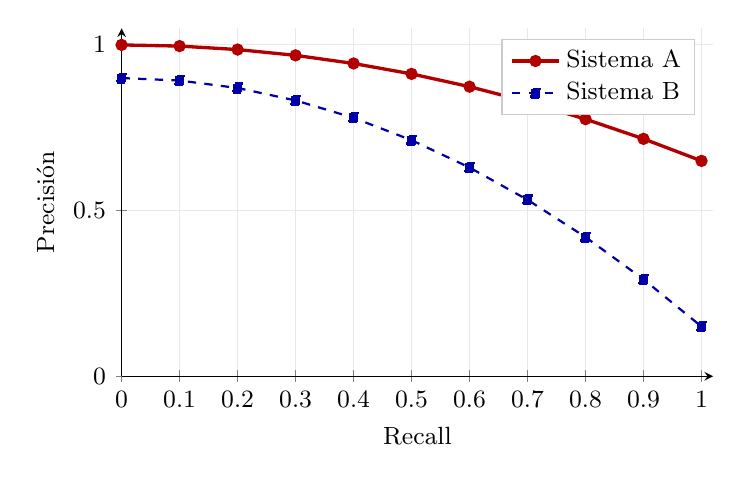
\begin{tikzpicture}
    \begin{axis}[
      width=0.75\linewidth, height=6cm,
      xlabel={Recall}, ylabel={Precisión},
      xmin=0, xmax=1.02, ymin=0, ymax=1.05,
      xtick={0,0.1,0.2,0.3,0.4,0.5,0.6,0.7,0.8,0.9,1},
      axis lines=left,
      grid=major, grid style={gray!18},
      tick label style={font=\small},
      label style={font=\small},
      legend pos=north east,
      legend cell align=left,
      legend style={font=\small, draw=gray!40},
      domain=0:1, samples=11,
    ]
      \addplot[very thick, red!70!black, mark=*, mark size=1.6pt]
        {1 - 0.35*x^2};
      \addlegendentry{Sistema A}
      \addplot[thick, blue!65!black, dashed, mark=square*,
               mark size=1.6pt] {0.9 - 0.75*x^2};
      \addlegendentry{Sistema B}
    \end{axis}
  \end{tikzpicture}

  
\end{figure}

\begin{ojo}
    La precisión casi siempre baja conforme sube el recall. Para
    recuperar más documentos relevantes hay que bajar el umbral, y al
    bajarlo entran también más irrelevantes. Ese compromiso es lo que
    la curva dibuja.
\end{ojo}

% =====================================================================

\subsection*{MAP}

\emph{Mean average precision} es de las medidas más usadas. Para cada
consulta se promedia la precisión medida justo en las posiciones donde
apareció un documento relevante, y después se promedian esas
consultas:
\[
    \mathrm{AP}(q) = \frac{1}{R} \sum_{k=1}^{n} P@k \cdot
    \mathrm{rel}(k) ,
    \qquad
    \mathrm{MAP} = \frac{1}{|Q|} \sum_{q \in Q} \mathrm{AP}(q) ,
\]
donde $R$ es el número de documentos relevantes, $n$ el tamaño del
ranking y $\mathrm{rel}(k)$ vale $1$ si el documento en la posición
$k$ es relevante y $0$ si no.

Esa suma es una aproximación discreta del área bajo la curva de
recall-precisión: cada término aporta el pedazo que corresponde a un
documento relevante.

\begin{figure}[htbp]
  \centering
  \begin{tikzpicture}
    \begin{axis}[
      width=0.75\linewidth, height=6cm,
      xlabel={Recall}, ylabel={Precisión},
      xmin=0, xmax=1.02, ymin=0, ymax=1.05,
      xtick={0,0.1,0.2,0.3,0.4,0.5,0.6,0.7,0.8,0.9,1},
      axis lines=left,
      grid=major, grid style={gray!18},
      tick label style={font=\small},
      label style={font=\small},
      domain=0:1, samples=11,
    ]
      \addplot[draw=none, fill=fondoIdea, opacity=0.9]
        {1 - 0.35*x^2} \closedcycle;
      \addplot[very thick, red!70!black, mark=*, mark size=1.6pt]
        {1 - 0.35*x^2};
      \node[font=\small, text=acento] at (axis cs:0.45,0.4)
        {área $\approx$ AP};
    \end{axis}
  \end{tikzpicture}
  \caption{La average precision de una consulta es el área bajo su
    curva de recall-precisión.}
  \label{fig:area-map}
\end{figure}

\subsubsection*{AP como suma de Riemann}

La correspondencia con el área no es una analogía suelta, la suma que
define AP es literalmente una suma de Riemann. Si la consulta tiene
$R$ documentos relevantes, cada uno que aparece sube el recall en
exactamente $1/R$, así que le toca un rectángulo de ese ancho y de
altura $P@k$. Sumar las áreas de los rectángulos es calcular
\[
    \mathrm{AP}(q) = \sum_{k=1}^{n}
    \underbrace{\vphantom{\frac{1}{R}} P@k \cdot \mathrm{rel}(k)}
               _{\text{altura}} \cdot
    \underbrace{\frac{1}{R}}_{\text{ancho}} .
\]

\begin{figure}[htbp]
  \centering
  \begin{tikzpicture}
    \begin{axis}[
      width=0.75\linewidth, height=6cm,
      xlabel={Recall}, ylabel={Precisión},
      xmin=0, xmax=1.02, ymin=0, ymax=1.05,
      xtick={0,0.1,0.2,0.3,0.4,0.5,0.6,0.7,0.8,0.9,1},
      axis lines=left,
      grid=major, grid style={gray!18},
      tick label style={font=\small},
      label style={font=\small},
      domain=0:1, samples=11,
    ]
      \addplot[ybar interval, fill=fondoIdea, draw=acento!55,
               opacity=0.9] {1 - 0.35*x^2};
      \addplot[very thick, red!70!black, mark=*, mark size=1.6pt]
        {1 - 0.35*x^2};
      % El ancho de un rectangulo es 1/R
      \draw[<->, acento, thin]
        (axis cs:0.5,0.12) -- (axis cs:0.6,0.12);
      \node[font=\footnotesize, text=acento, anchor=north]
        at (axis cs:0.55,0.11) {$1/R$};
      \node[font=\footnotesize, text=acento, anchor=west]
        at (axis cs:0.62,0.45) {altura $= P@k$};
    \end{axis}
  \end{tikzpicture}
  \caption{Cada documento relevante aporta un rectángulo de ancho
    $1/R$ y altura $P@k$. La suma de sus áreas es AP, con $R = 10$
    en el dibujo.}
  \label{fig:riemann-ap}
\end{figure}

\begin{ojo}
    Por eso AP no es el promedio de las precisiones de todo el
    ranking, sino solo de las posiciones donde hubo un relevante. Las
    demás posiciones no aportan rectángulo, porque no mueven el
    recall.
\end{ojo}

\subsubsection*{Ventajas y desventajas}

\textbf{A favor:}
\begin{itemize}[itemsep=0.1em]
    \item Es un solo valor, así que compara sistemas de un vistazo
    \item Se ajusta muy bien y no se fija tanto en las colas del
          ranking
    \item Es muy buena para métricas binarias, o sea cuando un
          documento simplemente es relevante o no lo es
\end{itemize}

\textbf{En contra:}
\begin{itemize}[itemsep=0.1em]
    \item No es tan buena para \emph{ratings} numéricos de grano
          fino, porque asume que todos los relevantes son igualmente
          relevantes, y eso no es cierto
\end{itemize}

\begin{pendiente}
    Preguntas que dejo el Dr para la sig clase: 
    \begin{itemize}
        \item pq todo lo que recupera un sistema de IR no es relevante?
        \item pq es difícil tener $100$ de recall?
        \item ideas para solucionarlo?
    \end{itemize}
\end{pendiente}

\newpage
% =====================================================================

\clase{Expansión de consultas y clustering}{7 de septiembre de 2026}

\begin{quick_sum}
    Arrancamos respondiendo las tres preguntas que quedaron pendientes
    de la clase pasada, y las tres tienen la misma raíz: la consulta es
    ambigua. De ahí salió la expansión de consultas, con sus tres vías
    (tesauros, retroalimentación del usuario y automática), el método
    de Rocchio y la semántica distribucional. Cerramos con clustering,
    que ataca el mismo problema pero del lado del resultado.
\end{quick_sum}

\subsection*{Por qué no se llega al 100}

Las tres preguntas que dejó el Dr. la clase pasada se responden con lo
mismo.

Es difícil tener 100 de precisión porque la consulta es ambigua. Basta
imaginar una consulta de una sola palabra: el sistema no tiene con qué
saber a cuál de sus sentidos se refiere el usuario, así que devuelve
documentos de todos, y los que sobran cuentan como error.

Es difícil tener 100 de recall por la misma razón. Si la consulta dice
\emph{coche} y el documento relevante dice \emph{automóvil}, el sistema
no los empata y ese documento se queda fuera.

\begin{idea}
    La salida es ser lo más específico posible en la consulta. El
    problema es que el usuario no sabe serlo: no conoce la colección ni
    el vocabulario con el que está escrita. Entonces el sistema lo hace
    por él, y eso es la expansión de consultas.
\end{idea}

\subsection*{Expansión de consultas}

Expandir una consulta es agregarle términos que el usuario no escribió
pero que apuntan a lo mismo que quiso decir: sinónimos, variantes
morfológicas, términos relacionados. La consulta original no se
sustituye, se le suman términos para que empate con más documentos
relevantes.

Sirve sobre todo para el recall, que es lo que la ambigüedad rompe
primero. El riesgo va en la otra dirección: cada término que se agrega
puede traer documentos que no vienen al caso, y eso baja la precisión.

Hay tres vías para decidir qué términos agregar:

\begin{itemize}[itemsep=0.2em]
    \item \textbf{Tesauros.} Un recurso externo ya construido, que dice
          qué palabras se relacionan con cuáles.
    \item \textbf{Retroalimentación del usuario.} Se le pregunta cuáles
          de los resultados le sirvieron y se aprende de ahí.
    \item \textbf{Expansión automática.} Las asociaciones se sacan de
          la propia colección, sin recurso externo ni usuario.
\end{itemize}

\subsubsection*{Basada en tesauros}

A cada término de la consulta se le agregan sus sinónimos y términos
relacionados según un tesauro, que puede ser general, como WordNet, o
del dominio.

Incrementa el recall, porque la consulta empieza a empatar con
documentos escritos con otro vocabulario. Pero baja la precisión, y la
razón es que el tesauro no sabe de cuál sentido se está hablando: si la
consulta trae \emph{banco}, le agrega lo de la institución financiera y
lo del asiento por igual.

\subsubsection*{Retroalimentación de relevancia}

El sistema devuelve una primera tanda de resultados, el usuario marca
cuáles le sirvieron y cuáles no, y con eso el sistema arma una consulta
nueva y vuelve a buscar.

La ventaja es que la evidencia viene del usuario, que es el único que
sabe qué necesita. La desventaja es que hay que pedírsela, y en un
buscador real casi nadie se toma la molestia.

\subsubsection*{Método de Rocchio}

Es la forma estándar de aplicar esa retroalimentación. Como todo son
vectores, la consulta se puede mover en el espacio: la idea es
acercarla a los documentos que el usuario marcó como relevantes y
alejarla de los que marcó como irrelevantes.

\[
    \vec{q}_m = \alpha\, \vec{q}_0
    + \beta\, \frac{1}{\abs{D_r}} \sum_{\vec{d} \in D_r} \vec{d}
    - \gamma\, \frac{1}{\abs{D_{nr}}} \sum_{\vec{d} \in D_{nr}} \vec{d}
\]

donde $\vec{q}_0$ es la consulta original, $D_r$ y $D_{nr}$ son los
conjuntos de documentos marcados como relevantes e irrelevantes, y
$\alpha$, $\beta$ y $\gamma$ pesan cuánto cuenta cada parte.

\begin{ojo}
    En la práctica $\beta > \gamma$. La evidencia positiva es más
    confiable que la negativa: que al usuario le haya servido un
    documento dice mucho, que no le haya servido puede deberse a que ya
    lo conocía o a que no lo abrió.
\end{ojo}

\subsubsection*{Retroalimentación pseudo relevante}

Igual que la anterior, pero sin preguntarle nada al usuario: se asume
que los primeros $n$ resultados son relevantes y se aplica Rocchio con
ellos.

Funciona bien cuando la primera tanda ya es decente. Cuando no lo es,
refuerza el error: la consulta se mueve hacia documentos equivocados y
la segunda tanda sale peor que la primera.

\subsection*{Semántica distribucional}

La tercera vía, la automática. En lugar de un tesauro externo o del
usuario, las asociaciones entre palabras salen de la propia colección.

Se parte de la matriz de términos contra documentos y se multiplica por
su transpuesta. El resultado es una matriz cuadrada de términos contra
términos, donde cada celda dice en cuántos contextos aparecen juntas
dos palabras.

\[
    C = A A^{T},
    \qquad
    A \in \R^{|V| \times |D|},
    \qquad
    C \in \R^{|V| \times |V|}
\]

\begin{idea}
    El tamaño del contexto cambia qué tipo de relación sale. Con un
    contexto grande se correlacionan palabras relacionadas por tema:
    médico con hospital. Con un contexto chico la correlación se acerca
    a la sinonimia, porque dos palabras rodeadas de las mismas pocas
    palabras suelen ser intercambiables.
\end{idea}

\subsection*{Clustering en recuperación de información}

Todo lo anterior ataca la ambigüedad sobre la marcha, antes de buscar.
El clustering la ataca del otro lado, en el momento de presentar el
resultado: se agrupan los resultados, por ejemplo por tema, y el
usuario escoge el grupo que le interesa. Ahí desambigua él, sin tener
que reescribir la consulta.

\begin{idea}
    \textbf{Hipótesis del cluster:} los documentos que caen en el mismo
    grupo se comportan de forma similar respecto a la relevancia. Si
    uno sirve para una necesidad de información, es probable que los
    demás del grupo también.
\end{idea}

Tiene dos usos principales:

\begin{itemize}[itemsep=0.2em]
    \item \textbf{Clustering de la colección.} Se agrupa antes de
          buscar. Da más eficiencia, porque la búsqueda se restringe a
          los grupos prometedores en vez de recorrer todo, y tiende a
          mejorar el recall.
    \item \textbf{Clustering de resultados.} Se agrupa lo que se va a
          devolver. No cambia qué se recuperó, cambia cómo se presenta,
          y con eso la información le llega al usuario de forma más
          efectiva.
\end{itemize}

\newpage
% =====================================================================



\clase{Representaciones más allá de las palabras}{9 de septiembre de 2026}

\begin{quick_sum}
    En esta clase impartió el Dr. Aurelio. Vimos repaso de conceptos que ya habíamos 
    visto antes, como la ambigüedad y los problemas de sinonimia y polisemia, y cómo 
    afectan la recuperación de información. 
    También se introdujo la pregunta de fondo del indexado: cuál es la mejor unidad 
    de representación para un documento y el POS tagging
\end{quick_sum}

\subsection*{Repaso: ambigüedad}

La ambigüedad es la condición donde una información puede entenderse o
interpretarse en más de un sentido. El contexto la mitiga, no la
elimina.

\begin{itemize}[itemsep=0.2em]
    \item \textbf{Léxica.} Palabras o frases con más de un significado
          posible: \textit{banco}, \textit{gato}.
    \item \textbf{Sintáctica.} La oración se puede parsear de varias
          formas, y cada árbol da una interpretación distinta.
    \item \textbf{Semántica.} El significado de una palabra o concepto
          es vago o queda abierto, aunque la sintaxis sea clara.
\end{itemize}

\subsubsection*{Qué subyace: sinonimia y polisemia}

Detrás de la ambigüedad hay dos problemas del lenguaje natural, y cada
uno rompe una métrica diferente.

\begin{center}
\begin{tabular}{lll}
    \toprule
    \textbf{Problema} & \textbf{Qué es} & \textbf{Qué degrada} \\
    \midrule
    Sinonimia & Varias palabras, un significado & Recall \\
    Polisemia & Una palabra, varios significados & Precisión \\
    \bottomrule
\end{tabular}
\end{center}

\begin{idea}
    La sinonimia baja el recall porque el documento relevante usa otra
    palabra y nunca se recupera. La polisemia baja la precisión porque
    la palabra empata con documentos de otro sentido y sí se recupera,
    pero sobra. Son direcciones opuestas, por eso no hay una sola
    solución que arregle las dos.
\end{idea}

\subsection*{Indexado de documentos}

El objetivo del indexado es encontrar los significados importantes de
un documento y construir con ellos una representación interna. Lo que
no se indexe no existe para el sistema.

Tres factores para juzgar una representación:

\begin{itemize}[itemsep=0.2em]
    \item \textbf{Precisión semántica.} Qué tan bien captura el
          significado.
    \item \textbf{Exhaustividad.} Si cubre todo el contenido del
          documento o solo una parte.
    \item \textbf{Manejabilidad.} Qué tan fácil le resulta a la
          computadora manipularla.
\end{itemize}

\subsubsection*{Cuál es la mejor unidad de representación}

\begin{center}
\begin{tabular}{lll}
    \toprule
    \textbf{Unidad} & \textbf{Cobertura} & \textbf{Precisión} \\
    \midrule
    Caracter  & Total    & Nula \\
    Palabra   & Buena    & Baja \\
    Frase     & Pobre    & Mayor \\
    Concepto  & Pobre    & Alta \\
    \bottomrule
\end{tabular}
\end{center}

\begin{idea}
    Ninguna gana. Al subir de unidad se gana precisión y se pierde
    cobertura: hay pocas frases y menos conceptos, así que casi nada
    empata. Al bajar pasa lo contrario, todo empata y nada discrimina.
    Por eso el modelo de espacio vectorial se quedó en la palabra: es
    el punto donde las dos curvas todavía se cruzan.
\end{idea}

\subsection*{Etiquetado gramatical (POS tagging)}

Tarea del procesamiento de lenguaje que consiste en asignarle a cada
palabra de una oración la categoría gramatical que asume \emph{en esa
secuencia}, no la que tendría aislada.

\begin{center}
\begin{tabular}{ll}
    \toprule
    \textbf{Entrada} & Una cadena de palabras más un conjunto de
                       etiquetas \\
    \textbf{Salida}  & Una sola etiqueta, la mejor, para cada palabra \\
    \bottomrule
\end{tabular}
\end{center}

La salida es una secuencia única: el etiquetador no propone
alternativas, se compromete con una.

\begin{ejemplo}
    Sobre una oración de la colección Time:
    \begin{center}
    \begin{tabular}{llllll}
        \toprule
        \textit{The} & \textit{allies} & \textit{saw} &
        \textit{the} & \textit{first} & \textit{outlines} \\
        DT & NNS & VBD & DT & JJ & NNS \\
        \bottomrule
    \end{tabular}
    \end{center}
    \textit{The} sale determinante, \textit{saw} verbo en pasado.
    Fuera de contexto \textit{saw} también es el sustantivo
    \textit{sierra}, y es justo la ambigüedad léxica que el etiquetado
    resuelve usando la secuencia.
\end{ejemplo}

\subsubsection*{Los conjuntos de etiquetas}

Los dos de referencia salen de sendos corpus anotados a mano. El de
\textbf{Brown} es el grande, del orden de 87 etiquetas, con
distinciones muy finas. El de \textbf{Penn Treebank} lo simplificó a 36
categorías gramaticales, más los signos de puntuación, y es el que se
usa por omisión hoy.

\begin{center}
\begin{tabular}{lll}
    \toprule
    \textbf{Etiqueta} & \textbf{Categoría} & \textbf{Ejemplo} \\
    \midrule
    NN, NNS   & Sustantivo singular, plural  & \textit{force, allies} \\
    NNP       & Nombre propio                & \textit{Kennedy} \\
    VB, VBD   & Verbo base, pasado           & \textit{help, saw} \\
    VBG, VBN  & Gerundio, participio         & \textit{suppressing} \\
    JJ        & Adjetivo                     & \textit{nuclear} \\
    RB        & Adverbio                     & \textit{finally} \\
    DT        & Determinante                 & \textit{the} \\
    IN        & Preposición                  & \textit{after} \\
    PRP       & Pronombre personal           & \textit{they} \\
    CD        & Número cardinal              & \textit{1960} \\
    \bottomrule
\end{tabular}
\end{center}

\begin{observacion}
    El etiquetado gramatical se empezó a trabajar en los años sesenta,
    en la misma época que el corpus de Brown.
\end{observacion}



\newpage
% =====================================================================



\clase{Indexado más allá de la palabra}{14 de septiembre de 2026}

\begin{quick_sum}
    Se cerró el etiquetado gramatical con las dos formas de resolverlo,
    la de la etiqueta más frecuente y la de modelos ocultos de Markov,
    y con el veredicto de para qué sirve en indexado.
    De ahí salieron las otras dos propuestas para representar un
    documento con algo distinto de la palabra suelta: las unidades
    compuestas (frases, entidades nombradas, n-gramas, secuencias
    frecuentes maximales) y el indexado por sentidos.
\end{quick_sum}

\subsection*{Cómo se resuelve el etiquetado}

\subsubsection*{Primer enfoque: la etiqueta más frecuente}

A cada palabra se le asigna la etiqueta que más veces recibe en un
corpus anotado. Si $w$ admite las etiquetas $t_1, \ldots, t_k$, se
escoge
\[
    \hat{t}(w) = \operatorname*{arg\,max}_{t_i} P(t_i \mid w) ,
    \qquad
    P(t_i \mid w) = \frac{C(t_i, w)}{C(w)} ,
\]
donde $C(t_i, w)$ es el número de veces que $w$ aparece etiquetada
$t_i$ en el corpus. El contexto no entra en la cuenta: la decisión es
la misma en toda oración donde aparezca $w$.

Aun así acierta alrededor del $91$ por ciento en inglés. La razón es
que la mayoría de las palabras no son ambiguas, y las que sí lo son
tienen una distribución muy sesgada hacia una de sus etiquetas. Por
ejemplo \textit{heat} se usa mucho más como sustantivo que como verbo,
así que este método siempre lo etiqueta sustantivo y casi siempre le
atina.

\begin{ojo}
    Ese $91$ por ciento es el piso contra el que se compara, no un
    buen resultado. Es una palabra mal etiquetada de cada once, y los
    errores no se reparten: caen justo sobre las palabras ambiguas,
    que son las frecuentes y las que más peso tienen en la
    interpretación.
\end{ojo}

\subsubsection*{Segundo enfoque: HMM tagging}

El etiquetado con modelos ocultos de Markov no decide palabra por
palabra, escoge la secuencia completa de etiquetas. Dada la secuencia
de palabras $w_1^n$, busca
\[
    \hat{t}_1^n
    = \operatorname*{arg\,max}_{t_1^n} P(t_1^n \mid w_1^n)
    = \operatorname*{arg\,max}_{t_1^n} P(w_1^n \mid t_1^n)\, P(t_1^n) ,
\]
donde la segunda igualdad es la regla de Bayes, quitando $P(w_1^n)$
porque es la misma para todas las secuencias candidatas y no cambia
cuál gana.

Así como está no se puede calcular, hay $|T|^n$ secuencias posibles.
Se meten dos suposiciones:

\begin{itemize}[itemsep=0.2em]
    \item \textbf{Emisión.} Cada palabra depende solo de su propia
          etiqueta, no de las vecinas:
          $P(w_1^n \mid t_1^n) \approx \prod_i P(w_i \mid t_i)$.
    \item \textbf{Transición.} Cada etiqueta depende solo de la
          anterior, o sea un bigrama:
          $P(t_1^n) \approx \prod_i P(t_i \mid t_{i-1})$.
\end{itemize}

Con las dos, el criterio queda
\[
    \hat{t}_1^n = \operatorname*{arg\,max}_{t_1^n}
                  \prod_{i=1}^{n} P(w_i \mid t_i)\,
                                  P(t_i \mid t_{i-1}) .
\]

Las dos probabilidades se estiman contando sobre el corpus anotado,
igual que antes. Y para no enumerar las $|T|^n$ secuencias se usa
Viterbi, programación dinámica que resuelve el máximo en
$O(n \cdot |T|^2)$.

\begin{ejemplo}
    En \textit{to heat the water}, el método de la etiqueta más
    frecuente pone \textit{heat} como sustantivo, porque ese es su uso
    más común. El HMM lo corrige sin saber nada especial de
    \textit{heat}: la transición manda. Después de TO casi siempre
    viene un verbo en forma base, así que
    $P(\text{VB} \mid \text{TO})$ es órdenes de magnitud mayor que
    $P(\text{NN} \mid \text{TO})$, y el producto se voltea a favor de
    VB aunque la emisión
    $P(\text{heat} \mid \text{NN})$ sea la más grande de las dos.
\end{ejemplo}

\begin{idea}
    Ahí está la diferencia entre los dos enfoques. El primero pregunta
    qué es esta palabra normalmente. El segundo pregunta qué secuencia
    de etiquetas hace más probable a la oración entera, y por eso
    puede ir contra la etiqueta favorita de una palabra cuando el
    contexto lo pide.
\end{idea}

\subsubsection*{Sirve el POS para indexar?}

Indexar con la etiqueta pegada al término separa \textit{saw} verbo de
\textit{saw} sustantivo, y con eso sube la precisión. Pero baja el
recall: un documento que usa la palabra con la otra etiqueta deja de
empatar, aunque hable de lo mismo.

\begin{ojo}
    El veredicto de la clase fue que no vale la pena como técnica de
    indexado por sí sola, ni siquiera si el etiquetado se hace a mano.
    El límite no es la calidad del etiquetador, es el intercambio:
    lo que gana en precisión lo paga en recuerdo. El POS tagging se
    queda como paso intermedio, insumo para extraer frases, no como el
    índice mismo.
\end{ojo}

\subsection*{Segunda propuesta: unidades compuestas}

Usar palabras sueltas como términos de indexado da buena exhaustividad
y especificidad pobre: se cubre todo el documento, pero cada término
discrimina poco. Y hay combinaciones cuyo significado no se recupera
separando las palabras, \textit{apple pie} no es una manzana más un
pastel.

De ahí la idea de usar términos de indexado de más de una palabra,
para reducir la ambigüedad.

\begin{ejemplo}
    Sobre \textit{this apple pie looks good and is a real treat}:
    \begin{center}
    \begin{tabular}{ll}
        \toprule
        \textbf{Relación} & \textbf{Término} \\
        \midrule
        Adjetivo, sustantivo   & \textit{real treat} \\
        Sustantivo, sustantivo & \textit{apple pie} \\
        Sujeto, verbo          & \textit{pie looks} \\
        Verbo, objeto          & \textit{is treat} \\
        \bottomrule
    \end{tabular}
    \end{center}
\end{ejemplo}

La complicación es de dónde salen: hay que extraerlas del texto ya
etiquetado con POS o del árbol sintáctico, y el análisis sintáctico
completo es caro.

La alternativa barata es el \textbf{chunking}, o análisis superficial.
En vez de construir el árbol entero, reconoce bloques no recursivos
(sobre todo sintagmas nominales) con patrones sobre las etiquetas POS.
La operación complementaria es el \textbf{chinking}, que define qué
sacar de un bloque ya formado en lugar de qué meter.

\subsubsection*{Entidades nombradas}

Son las entidades que el texto menciona por nombre. Las tres clases
aceptadas son personas, lugares y organizaciones. Suelen agregarse
fecha, hora, medidas, correos y direcciones.

La ambigüedad sigue presente aunque se trabaje con entidades: un
nombre como \textit{Charlie Kirk} puede ser una persona o un lugar,
porque a los lugares se les pone nombre de persona.

Se procesan en dos pasos:

\begin{enumerate}[itemsep=0.2em]
    \item \textbf{Identificación.} Detectar los límites, dónde empieza
          y dónde termina la entidad nombrada.
    \item \textbf{Clasificación.} Asignarle una de las categorías
          predefinidas.
\end{enumerate}

Cómo se ha atacado, en orden histórico:

\begin{center}
\begin{tabular}{>{\raggedright\arraybackslash}p{3.1cm}
                >{\raggedright\arraybackslash}p{5.1cm}
                >{\raggedright\arraybackslash}p{5.1cm}}
    \toprule
    \textbf{Enfoque} & \textbf{Cómo} & \textbf{Limitación} \\
    \midrule
    Reglas basadas en conocimiento &
    Expertos se sientan a escribir patrones y a etiquetar a mano &
    No escala, y se rehace entero para cada dominio \\
    \addlinespace
    Aprendizaje automático y estadística (HMM, CRF) &
    Explota rasgos de los elementos de interés: mayúsculas, patrones,
    POS, prefijos y sufijos &
    Requiere corpus extensos ya anotados \\
    \addlinespace
    Aprendizaje profundo y transformers (BERT, RoBERTa) &
    Embeddings contextuales, la representación se aprende sola, sin
    ingeniería manual de rasgos &
    Mucho cómputo y conjuntos grandes para el ajuste fino por
    dominio \\
    \bottomrule
\end{tabular}
\end{center}

\subsubsection*{N-gramas}

Un n-grama es una subsecuencia de $n$ términos de una secuencia dada.
Sobre \textit{apple pie looks good}, los bigramas son
\textit{apple pie}, \textit{pie looks} y \textit{looks good}.

Lo que los hace atractivos:

\begin{itemize}[itemsep=0.2em]
    \item Se calculan fácil, una pasada con una ventana deslizante.
          No hacen falta etiquetador ni analizador sintáctico.
    \item Se pueden combinar n-gramas de distinto tamaño, y eso da
          flexibilidad al momento de buscar: la consulta empata con la
          granularidad que tenga.
\end{itemize}

El problema es la alta dimensionalidad. El número de n-gramas crece
muy por encima del tamaño del vocabulario, y el índice se vuelve
inmanejable.


\subsubsection*{Secuencias frecuentes maximales}

Otro enfoque que también sale de las frecuencias. Una secuencia es
frecuente si aparece en al menos cierto número de documentos de la
colección, y es \textbf{maximal} si no está contenida en ninguna otra
secuencia frecuente más larga.

\begin{ejemplo}
    Si \textit{united states of america} es frecuente, entonces
    \textit{united states} también lo es, porque está contenida en
    ella. Solo se queda la larga.
\end{ejemplo}

Esa poda es justo su fortaleza: el índice que forma es muy compacto.
La extracción de las MFS se hace normalmente combinando métodos
bottom-up con métodos voraces.

\subsubsection*{Funciona el indexado compuesto?}

El veredicto es mixto. Mejora los resultados en niveles bajos de
recuerdo, o sea en la cabeza del ranking, los primeros documentos que
regresa el sistema. Pero conforme la colección crece, la anotación de
entidades nombradas se vuelve el cuello de botella y la ganancia se
diluye.

\begin{idea}
    La recomendación de la clase no es reemplazar la bolsa de
    palabras. Es considerar las frases como términos suplementarios
    del espacio vectorial, encima de las palabras, no en lugar de
    ellas.
\end{idea}

\subsection*{Tercera propuesta: indexado por sentidos}

La tercera idea es ir más allá del empatamiento de términos, hacia el
indexado por sentidos. La motivación son la sinonimia y la polisemia
de la clase pasada: empatar cadenas de caracteres no arregla ninguna
de las dos, porque una es un problema de recall y la otra de
precisión. Lo que se busca entonces es capturar conceptos.

Pero qué es un sentido? Es uno de los significados de una palabra.
Las palabras tienen más de un significado, y cuál de ellos aplica lo
decide el contexto.





\newpage
% =====================================================================
%  Clase 11 - Desambiguacion e indexado conceptual
% =====================================================================

\clase{Desambiguación e indexado conceptual}{21 de septiembre de 2026}

\begin{quick_sum}
    Continuación del indexado por sentidos. Se separó el significado
    del sentido, se definió la desambiguación del sentido de las
    palabras y se contrastó con la discriminación. De ahí salieron el
    proceso de tres pasos, los dos enfoques para resolverlo, WordNet
    como inventario de sentidos y el algoritmo de Lesk. Al final entró
    la cuarta propuesta de indexado, la conceptual, con DOR.
\end{quick_sum}

\subsection*{Significado y sentido}

Se usan casi como sinónimos, pero no son lo mismo:

\begin{itemize}[itemsep=0.2em]
    \item El \textbf{significado} es lo que está en el diccionario o
          en el tesauro. Es una lista fija, escrita de antemano, que
          no depende del texto que se esté procesando.
    \item El \textbf{sentido} lo da el contexto, los términos que
          rodean a la palabra en ese documento. Es lo que selecciona
          cuál de los significados aplica.
\end{itemize}

Indexar así cambia la tabla del índice: una palabra deja de tener una
entrada y pasa a tener dos o más, una por cada sentido.
\textit{bank} como orilla del río y \textit{bank} como institución
financiera pasan a ser términos de indexado distintos, aunque la
cadena de caracteres sea la misma.

\begin{idea}
    Ese desdoblamiento es lo que ataca la polisemia: dos documentos
    que comparten la cadena pero no el sentido dejan de empatar. Y si
    además los sinónimos se colapsan en una sola entrada, se ataca la
    sinonimia. Las dos de un golpe, que es justo lo que no logra el
    empatamiento de cadenas.
\end{idea}

\subsection*{Desambiguación y discriminación}

La \textbf{desambiguación del sentido de las palabras} (WSD, por
\textit{word sense disambiguation}) es la tarea de seleccionar el
sentido correcto de una palabra a partir de un conjunto predefinido.
El inventario de sentidos existe antes de ver el texto.

La \textbf{discriminación} está relacionada, pero es diferente. La
pregunta aquí es otra: dado un conjunto de textos, qué sentidos
distintos surgen en ellos. No hay inventario, y un sistema encaminado
a la discriminación tiene que distinguir los sentidos con esa base de
documentos. Los sentidos son la salida, no la entrada.

\begin{center}
\begin{tabular}{>{\raggedright\arraybackslash}p{2.3cm}
                >{\raggedright\arraybackslash}p{5.4cm}
                >{\raggedright\arraybackslash}p{5.4cm}}
    \toprule
    & \textbf{Desambiguación} & \textbf{Discriminación} \\
    \midrule
    Inventario &
    Predefinido y externo, el mismo para toda colección &
    Se induce de los datos, cambia con la colección \\
    \addlinespace
    Salida &
    Una etiqueta de sentido por ocurrencia &
    Grupos de ocurrencias, sin nombre que los identifique \\
    \addlinespace
    Método &
    Clasificación &
    Agrupamiento \\
    \addlinespace
    Necesita &
    Un recurso léxico, o un corpus ya anotado &
    Solo los documentos de la colección \\
    \bottomrule
\end{tabular}
\end{center}

\subsection*{El proceso de WSD}

\subsubsection*{1. Elegir un inventario de sentidos}

Es la decisión que condiciona todo lo demás, porque fija cuáles son
los sentidos posibles. Un sentido que no esté en el inventario no se
puede asignar nunca, por bueno que sea el método.

Las opciones van de un diccionario o un tesauro a una base como
WordNet o a una ontología del dominio. Lo que se negocia al escoger es
la \textbf{granularidad}:

\begin{itemize}[itemsep=0.2em]
    \item Un inventario fino distingue matices, y ahí la tarea se
          vuelve tan difícil que ni los anotadores humanos coinciden
          entre sí.
    \item Uno grueso separa solo los sentidos muy distintos, los
          homógrafos. Da acuerdo alto, pero captura menos.
\end{itemize}

Para recuperación conviene el grueso: interesan los sentidos que
cambian el tema del documento, no los que cambian el matiz.

\subsubsection*{2. Diseñar y aplicar el procedimiento}

Se decide el alcance y el método. El alcance puede ser de dos tipos:

\begin{itemize}[itemsep=0.2em]
    \item \textbf{Todas las palabras}. Etiquetar cada palabra de
          contenido del texto. Es lo que hace falta para indexar una
          colección entera.
    \item \textbf{Muestra léxica}. Solo unas cuantas palabras
          objetivo, escogidas de antemano. Es el escenario de los
          concursos de evaluación.
\end{itemize}

El método cae en una de dos familias, basada en conocimiento o basada
en aprendizaje automático, que van más abajo.

\subsubsection*{3. Evaluar el desempeño}

Hay dos maneras de medir, y no responden la misma pregunta:

\begin{itemize}[itemsep=0.2em]
    \item \textbf{In vitro}. La exactitud contra un corpus anotado a
          mano. Mide la tarea aislada.
    \item \textbf{In vivo}. Meter el desambiguador en el SRI y ver si
          sube el MAP. Es la que importa aquí, porque un
          desambiguador puede ser bueno y aun así no mover la
          recuperación.
\end{itemize}

Y hay dos referencias contra las cuales comparar el número que salga:

\begin{itemize}[itemsep=0.2em]
    \item El \textbf{piso}: asignar siempre el sentido más frecuente
          de la palabra. Es sorprendentemente difícil de superar,
          porque la distribución de sentidos está muy sesgada.
    \item El \textbf{techo}: el acuerdo entre anotadores humanos. Si
          dos personas solo coinciden el $75$ por ciento de las
          veces, no tiene sentido exigirle $90$ al sistema.
\end{itemize}

\subsection*{Los dos enfoques}

\subsubsection*{Basados en conocimiento}

Se apoyan en recursos léxicos ya construidos, diccionarios, tesauros
o redes semánticas, y no necesitan datos etiquetados. La información
sale del recurso, no de ejemplos.

Cómo deciden:

\begin{itemize}[itemsep=0.2em]
    \item \textbf{Traslape de glosas}. Comparar la definición de cada
          sentido con el contexto y quedarse con la que más palabras
          comparte. Es Lesk, que va abajo.
    \item \textbf{Métodos de grafo}. Armar el subgrafo de WordNet que
          conecta a los sentidos candidatos de todas las palabras de
          la oración y quedarse con los nodos mejor conectados.
    \item \textbf{Restricciones de selección}. Un verbo restringe la
          clase semántica de su objeto: \textit{comer} pide algo
          comestible, y con eso se descartan sentidos.
\end{itemize}

A favor tienen la cobertura: alcanzan cualquier palabra que el
recurso incluya, sin pagar anotación. En contra, dependen por
completo de la calidad y la cobertura de ese recurso.

\subsubsection*{Basados en aprendizaje automático}

Tratan la desambiguación como un problema de clasificación. Cada
ocurrencia se convierte en un vector de rasgos tomados de su
contexto, y un clasificador predice el sentido.

Los rasgos típicos salen de una ventana alrededor de la palabra
objetivo:

\begin{itemize}[itemsep=0.2em]
    \item La bolsa de palabras de la ventana, las $k$ palabras de
          cada lado sin importar el orden.
    \item Las colocaciones, o sea las palabras exactas en las
          posiciones $-1$, $+1$, $-2$, $+2$, que sí conservan el
          orden.
    \item La etiqueta gramatical de los vecinos, y las relaciones
          sintácticas si hay analizador.
\end{itemize}

Según cuántos datos etiquetados haya, hay tres variantes:

\begin{center}
\begin{tabular}{>{\raggedright\arraybackslash}p{3.0cm}
                >{\raggedright\arraybackslash}p{5.0cm}
                >{\raggedright\arraybackslash}p{5.0cm}}
    \toprule
    \textbf{Variante} & \textbf{Qué necesita} & \textbf{Qué entrega}
    \\
    \midrule
    Supervisada &
    Un corpus anotado con sentidos, palabra por palabra &
    La mejor exactitud de las tres \\
    \addlinespace
    No supervisada &
    Solo texto crudo &
    Grupos de ocurrencias, o sea discriminación, no
    desambiguación \\
    \addlinespace
    Semisupervisada &
    Unas cuantas ocurrencias semilla por sentido &
    Un clasificador que se amplía solo, etiquetando lo que ya
    reconoce con confianza \\
    \bottomrule
\end{tabular}
\end{center}

La semisupervisada se apoya en dos regularidades del lenguaje que se
cumplen casi siempre: un sentido por colocación, la palabra
acompañante fija el sentido, y un sentido por discurso, dentro de un
mismo documento la palabra conserva el sentido con el que apareció la
primera vez.

\begin{ojo}
    El cuello de botella del enfoque supervisado es la adquisición de
    conocimiento: hace falta un corpus anotado por cada palabra que
    se quiera desambiguar, anotar sentidos a mano es caro y los
    anotadores no siempre coinciden. Por eso el enfoque basado en
    conocimiento sigue vivo aunque sea menos exacto.
\end{ojo}

\subsection*{WordNet}

Es una base de datos léxica del inglés organizada en torno a los
significados de las palabras y a las relaciones semánticas entre
ellos. Incluye sustantivos, verbos, adjetivos y adverbios.

Su unidad no es la palabra. Las palabras con el mismo significado o
muy cercano se agrupan en un \textbf{synset}, un conjunto de
sinónimos, y cada synset representa un concepto particular. Los
synsets están conectados por relaciones semánticas.

\begin{center}
\begin{tabular}{>{\raggedright\arraybackslash}p{2.6cm}
                >{\raggedright\arraybackslash}p{5.2cm}
                >{\raggedright\arraybackslash}p{5.2cm}}
    \toprule
    \textbf{Relación} & \textbf{Qué liga} & \textbf{Ejemplo} \\
    \midrule
    Sinonimia & Las palabras dentro de un mismo synset &
    \textit{coche}, \textit{automóvil}, \textit{carro} \\
    \addlinespace
    Hiperonimia & Del caso al tipo general, es-un &
    \textit{perro} es un \textit{cánido} \\
    \addlinespace
    Hiponimia & La inversa, del tipo al caso &
    \textit{cánido} tiene por caso a \textit{perro} \\
    \addlinespace
    Holonimia & Del todo a la parte, tiene-parte &
    \textit{coche} tiene por parte a \textit{rueda} \\
    \addlinespace
    Meronimia & La inversa, de la parte al todo &
    \textit{rueda} es parte de \textit{coche} \\
    \addlinespace
    Antonimia & Opuestos, sobre todo entre adjetivos &
    \textit{caliente} y \textit{frío} \\
    \bottomrule
\end{tabular}
\end{center}

\subsubsection*{Hiperonimia}

$Y$ es hiperónimo de $X$ si todo $X$ es un tipo de $Y$. Es la
relación es-un, y lo importante es que es transitiva: si
\textit{perro} es un \textit{cánido} y \textit{cánido} es un
\textit{carnívoro}, entonces \textit{perro} es un \textit{carnívoro}.

Esa transitividad es la que organiza los sustantivos de WordNet en
una jerarquía con raíz única. Subiendo desde \textit{perro} se llega
a la raíz:

\begin{center}
    \textit{perro} $\to$ \textit{cánido} $\to$ \textit{carnívoro}
    $\to$ \textit{mamífero} $\to$ \textit{vertebrado} $\to$
    \textit{animal} $\to$ \textit{organismo} $\to$ \textit{entidad}
\end{center}

La relación inversa, bajando, es la hiponimia.

\subsubsection*{Holonimia}

$Y$ es holónimo de $X$ si $X$ es parte de $Y$. Es la relación
parte-de, vista desde el todo; vista desde la parte, la inversa, se
llama meronimia. WordNet distingue tres tipos:

\begin{itemize}[itemsep=0.2em]
    \item \textbf{Componente}. \textit{rueda} es parte de
          \textit{coche}.
    \item \textbf{Miembro}. \textit{árbol} es miembro de
          \textit{bosque}.
    \item \textbf{Sustancia}. \textit{oxígeno} es sustancia de
          \textit{agua}.
\end{itemize}

\begin{ojo}
    A diferencia de la hiperonimia, esta no se puede encadenar sin
    cuidado. La manija es parte de la puerta y la puerta es parte de
    la casa, pero decir que la manija es parte de la casa ya suena
    raro. La transitividad solo se sostiene dentro del mismo tipo de
    meronimia.
\end{ojo}

\begin{idea}
    Para indexar, lo que se gana con el synset es directo: los
    sinónimos se colapsan en una entrada, los sentidos de una
    polisémica se separan en varias, y la jerarquía de hiperónimos
    da una forma controlada de expandir la consulta. Si nada empata
    con \textit{sedán}, se sube un nivel a \textit{coche}. Es la
    expansión de consultas de la clase del $7$ de septiembre, pero
    con un recurso que dice a dónde subir en vez de adivinarlo de las
    coocurrencias.
\end{idea}

\subsection*{El algoritmo de Lesk}

Lesk (1986) es el representante clásico de los métodos basados en
conocimiento, y la idea cabe en una frase: el sentido correcto de una
palabra es aquel cuya definición comparte más palabras con el
contexto en el que la palabra aparece.

\begin{algorithm}[H]
\caption{Lesk simplificado}
\begin{algorithmic}[1]
\Procedure{Lesk}{$w$, $contexto$}
    \State $mejor \gets$ sentido más frecuente de $w$
    \State $mayor \gets 0$
    \For{cada sentido $s$ de $w$ en el inventario}
        \State $firma \gets$ palabras de la glosa y los ejemplos
                            de $s$
        \State $traslape \gets \abs{firma \cap contexto}$
        \If{$traslape > mayor$}
            \State $mayor \gets traslape$
            \State $mejor \gets s$
        \EndIf
    \EndFor
    \State \Return $mejor$
\EndProcedure
\end{algorithmic}
\end{algorithm}

La versión original de Lesk no compara la glosa contra el contexto,
compara las glosas entre sí: toma todas las palabras de contenido de
la ventana, considera todas las combinaciones de un sentido por
palabra y se queda con la combinación que maximiza el traslape entre
las glosas elegidas. Desambigua todas las palabras a la vez, y es
mucho más cara.

\begin{ejemplo}
    El caso clásico es la frase \textit{pine cone}. Las glosas del
    diccionario son:

    \textit{pine}
    \begin{enumerate}[itemsep=0.1em,label=\arabic*.]
        \item kinds of evergreen tree with needle-shaped leaves
        \item waste away through sorrow or illness
    \end{enumerate}

    \textit{cone}
    \begin{enumerate}[itemsep=0.1em,label=\arabic*.]
        \item solid body which narrows to a point
        \item something of this shape whether solid or hollow
        \item fruit of certain evergreen trees
    \end{enumerate}

    Con dos sentidos de \textit{pine} y tres de \textit{cone} hay
    seis combinaciones que revisar:

    \begin{center}
    \begin{tabular}{lll}
        \toprule
        \textbf{Combinación} & \textbf{Palabras en común} &
        \textbf{Traslape} \\
        \midrule
        \textit{pine} 1, \textit{cone} 1 & ninguna & $0$ \\
        \textit{pine} 1, \textit{cone} 2 & ninguna & $0$ \\
        \textit{pine} 1, \textit{cone} 3 &
        \textit{evergreen}, \textit{tree} & $2$ \\
        \textit{pine} 2, \textit{cone} 1 & ninguna & $0$ \\
        \textit{pine} 2, \textit{cone} 2 & ninguna & $0$ \\
        \textit{pine} 2, \textit{cone} 3 & ninguna & $0$ \\
        \bottomrule
    \end{tabular}
    \end{center}

    Gana la pareja \textit{pine} 1 con \textit{cone} 3: el árbol y su
    fruto, que es la lectura correcta. Las dos palabras quedaron
    desambiguadas al mismo tiempo.
\end{ejemplo}

\subsubsection*{Desventajas}

Son dos, y las dos se ven en el ejemplo:

\begin{enumerate}[itemsep=0.4em]
    \item \textbf{Son muchas combinaciones a analizar.} Con dos
          palabras fueron seis. Con una ventana de $k$ palabras de
          contenido donde cada una tiene $s$ sentidos en promedio,
          son $s^k$ combinaciones. Una oración de diez palabras de
          contenido con tres sentidos cada una ya da
          $3^{10} = 59\,049$ combinaciones que evaluar. Por eso en la
          práctica se usa la versión simplificada, que es lineal en
          el número de sentidos de la palabra objetivo.
    \item \textbf{Puede no haber suficiente traslape entre las
          definiciones.} Las glosas son cortas, una docena de
          palabras, y es muy común que dos definiciones correctas no
          compartan ni una. Cuando todos los traslapes dan cero el
          algoritmo no tiene con qué decidir y se cae al sentido más
          frecuente.
\end{enumerate}

Los dos parches habituales para lo segundo: expandir la firma de cada
sentido con las glosas de los synsets vecinos en WordNet, hiperónimos
e hipónimos incluidos, y pesar el traslape con idf para que las
palabras comunes no dominen la cuenta.

\begin{idea}
    La desambiguación es benéfica cuando las consultas son muy
    cortas. Dos o tres palabras no alcanzan para desambiguarse entre
    sí, y es justo ahí donde el sentido equivocado hace más daño. En
    una consulta larga los demás términos ya desambiguan solos y el
    desambiguador aporta poco. Con todo, la desambiguación sigue
    siendo un problema actual, no resuelto.
\end{idea}

\begin{ojo}
    Un desambiguador imperfecto puede dejar la recuperación peor de
    como estaba. Sanderson (1994) midió eso: por debajo de una
    exactitud cercana al $90$ por ciento, los errores de sentido
    meten más ruido del que quitan y conviene no desambiguar. Es el
    mismo intercambio del etiquetado gramatical de la clase pasada,
    lo que se gana en precisión se paga en recuerdo.
\end{ojo}

\subsection*{Cuarta propuesta: indexado conceptual}

La formulación del problema es que la bolsa de palabras ignora toda
la información semántica, trabaja solo con las formas superficiales
de las palabras. Esta cuarta representación busca el tipo conceptual.

El concepto está relacionado con el sentido, pero desde un punto de
vista práctico: no hace falta un inventario escrito por
lexicógrafos ni un desambiguador. La idea es representar los
documentos en función de las palabras que ocurren en ellos, y que la
semántica del documento se obtenga a partir de eso.

\begin{idea}
    Es un cambio de dónde viene el significado. En la propuesta
    anterior lo aportaba un recurso externo, WordNet. Aquí lo aporta
    la colección misma: dos palabras significan algo parecido si
    aparecen en los mismos documentos. Es la semántica distribucional
    de la clase del $7$ de septiembre, llevada al indexado.
\end{idea}

\subsubsection*{DOR}

La primera propuesta es \textbf{DOR}, representación por ocurrencia
en documentos (\textit{document occurrence representation}).

El giro está en qué se toma como concepto: cada documento de la
colección es una dimensión, un concepto primitivo. Una palabra se
describe entonces por los documentos en los que ocurre, y dos
palabras se parecen si ocurren en los mismos.

\begin{ojo}
    DOR es una representación de palabras, no de documentos. Lo que
    construye directamente es un vector por cada término del
    vocabulario. La representación del documento viene después, y es
    derivada.
\end{ojo}

El peso de la dimensión $d_j$ en la representación del término $t_i$
se calcula como el dual de tf-idf, intercambiando los papeles de
término y documento:
\[
    w_{ij} = \mathrm{tf}_{i,j} \cdot \log \frac{\abs{T}}{\abs{T_j}} ,
\]
donde $\abs{T}$ es el tamaño del vocabulario y $\abs{T_j}$ el número
de términos distintos que contiene $d_j$. La lectura es tf-idf al
revés: un documento que toca muchísimos términos distintos describe
mal cualquier concepto, igual que un término que aparece en
muchísimos documentos discrimina mal.

\subsubsection*{De palabras a documentos}

Con los vectores de palabra ya construidos, el documento se arma
sumando: la representación de un documento es la suma de los vectores
de las palabras que contiene. Las consultas se representan igual,
sumando los vectores de sus palabras.

El efecto sobre la matriz es el que importa. La matriz
palabra-documento, de $m \times n$, se convierte en una matriz
documento-documento, de $n \times n$, y esa segunda es la que se usa
como índice para la recuperación.

\begin{center}
\begin{tabular}{ccc}
    \textbf{Palabra-documento} & & \textbf{Documento-documento} \\
    \small representación de palabras & &
    \small índice para recuperación \\[0.7em]
    \begin{tabular}{c|cccc}
                 & $d_1$ & $d_2$ & $\cdots$ & $d_n$ \\
        \hline
        $t_1$    &       &          &       &       \\
        $t_2$    &       &          &       &       \\
        $\vdots$ &       & $w_{ij}$ &       &       \\
        $t_m$    &       &          &       &       \\
    \end{tabular}
    &
    \quad $\xrightarrow{\ \text{suma}\ }$ \quad
    &
    \begin{tabular}{c|cccc}
                 & $d_1$ & $d_2$ & $\cdots$ & $d_n$ \\
        \hline
        $d_1$    &       &          &       &       \\
        $d_2$    &       &          &       &       \\
        $\vdots$ &       & $w_{ij}$ &       &       \\
        $d_n$    &       &          &       &       \\
    \end{tabular}
\end{tabular}
\end{center}

\begin{ejemplo}
    Una colección de cuatro documentos, dos de fútbol y dos de
    medicina, con pesos crudos para que la cuenta se siga a mano:
    $d_1$ contiene \textit{gol} y \textit{equipo}, $d_2$
    \textit{gol} y \textit{árbitro}, $d_3$ \textit{virus} y
    \textit{fiebre}, y $d_4$ \textit{virus} y \textit{paciente}.

    Cada renglón de la matriz palabra-documento es el vector DOR de
    una palabra:

    \begin{center}
    \begin{tabular}{lcccc}
        \toprule
        & $d_1$ & $d_2$ & $d_3$ & $d_4$ \\
        \midrule
        \textit{gol}      & $1$ & $1$ & $0$ & $0$ \\
        \textit{equipo}   & $1$ & $0$ & $0$ & $0$ \\
        \textit{árbitro}  & $0$ & $1$ & $0$ & $0$ \\
        \textit{virus}    & $0$ & $0$ & $1$ & $1$ \\
        \textit{fiebre}   & $0$ & $0$ & $1$ & $0$ \\
        \textit{paciente} & $0$ & $0$ & $0$ & $1$ \\
        \bottomrule
    \end{tabular}
    \end{center}

    Sumando los vectores de las palabras de cada documento sale la
    matriz documento-documento:
    \begin{align*}
        d_1 &= (1,1,0,0) + (1,0,0,0) = (2,1,0,0) \\
        d_2 &= (1,1,0,0) + (0,1,0,0) = (1,2,0,0) \\
        d_3 &= (0,0,1,1) + (0,0,1,0) = (0,0,2,1) \\
        d_4 &= (0,0,1,1) + (0,0,0,1) = (0,0,1,2)
    \end{align*}

    Queda diagonal por bloques: los dos documentos de fútbol se
    parecen entre sí y no se parecen nada a los de medicina, y nadie
    tuvo que declarar cuáles eran los temas.

    Ahora la consulta \textit{equipo}, que se representa con el
    vector de esa palabra, $(1,0,0,0)$. Los cosenos contra los cuatro
    documentos son
    \[
        \cos(q, d_1) = \frac{2}{\sqrt{5}} = 0.894 ,
        \qquad
        \cos(q, d_2) = \frac{1}{\sqrt{5}} = 0.447 ,
    \]
    y cero contra $d_3$ y $d_4$.
\end{ejemplo}

\begin{idea}
    Lo interesante del ejemplo está en $d_2$: la palabra
    \textit{equipo} no aparece en $d_2$. Con la bolsa de palabras su
    similitud sería exactamente cero y ese documento no se
    recuperaría nunca. DOR lo trae porque \textit{equipo} y
    \textit{gol} coocurren en $d_1$, y \textit{gol} sí está en $d_2$.
    La conexión que en la propuesta anterior tenía que poner el
    diccionario, aquí la puso la colección.
\end{idea}

\begin{ojo}
    El costo es la dimensionalidad. El vector de una palabra tiene
    tantas componentes como documentos haya, así que la
    representación crece con la colección y no con el vocabulario. Y
    al sumar, los documentos dejan de ser dispersos: la matriz
    documento-documento se llena. Para una colección grande eso pesa
    más que el índice invertido de siempre.
\end{ojo}

\newpage
% =====================================================================
%  Clase 12 - Representaciones conceptuales
% =====================================================================

\clase{Representaciones conceptuales}{23 de septiembre de 2026}

\begin{quick_sum}
    Continuación del indexado conceptual. Después de DOR vino su
    pareja, TCOR, que describe cada palabra por las palabras con las
    que coocurre. Luego random indexing, una forma barata de construir
    bolsas de conceptos, qué tanto funcionan en IR y la
    representación más usada, LSI.
\end{quick_sum}

\subsection*{TCOR}

En WSD una palabra se representa por los términos que ocurren en su
contexto: el significado de una palabra lo transmiten las palabras
que suelen aparecer junto a ella. Esa es la base de \textbf{TCOR},
representación por coocurrencia de términos (\textit{term
co-occurrence representation}).

Cambia el concepto primitivo respecto a DOR. Allá cada documento era
una dimensión; aquí cada palabra del vocabulario lo es. La matriz es
palabra-palabra, de $m \times m$, y la celda $w_{ij}$ pesa la
coocurrencia de $t_i$ con $t_j$.

\begin{center}
\begin{tabular}{c|cccc}
             & $t_1$ & $t_2$ & $\cdots$ & $t_m$ \\
    \hline
    $t_1$    &       &          &       &       \\
    $t_2$    &       &          &       &       \\
    $\vdots$ &       & $w_{ij}$ &       &       \\
    $t_m$    &       &          &       &       \\
\end{tabular}
\end{center}

Las dos intuiciones sobre los pesos son las mismas de tf-idf, con
palabras en lugar de documentos:

\begin{itemize}[itemsep=0.3em]
    \item Entre más contextos compartan $t_i$ y $t_j$, más importa
          $t_j$ para caracterizar la semántica de $t_i$. Es el tf.
    \item Entre más palabras distintas acompañen a $t_j$, menos
          aporta a caracterizar a $t_i$. Es el idf: una palabra que
          aparece con todo no dice nada de nadie.
\end{itemize}

Juntas dan el peso
\[
    w_{ij} = \mathrm{tf}_{i,j} \cdot \log \frac{\abs{T}}{\abs{T_j}} ,
\]
donde $\mathrm{tf}_{i,j}$ es el número de contextos en que coocurren
$t_i$ y $t_j$, y $\abs{T_j}$ el número de términos distintos con los
que coocurre $t_j$.

Igual que DOR, TCOR es una representación de palabras. El documento
se obtiene sumando los vectores de sus palabras, y la consulta igual.
La matriz palabra-palabra se vuelve una matriz documento-palabra, de
$n \times m$, que es el índice para recuperar.

\begin{ejemplo}
    La misma colección de fútbol y medicina de DOR, con conteos crudos
    y el documento como contexto. Cada palabra coocurre consigo misma
    una vez, por eso la diagonal vale $1$. Los vectores de las palabras
    de fútbol, sobre las dimensiones (\textit{gol}, \textit{equipo},
    \textit{árbitro}, \textit{virus}, \textit{fiebre},
    \textit{paciente}), son
    \begin{align*}
        \textit{gol}     &= (1,1,1,0,0,0) \\
        \textit{equipo}  &= (1,1,0,0,0,0) \\
        \textit{árbitro} &= (1,0,1,0,0,0)
    \end{align*}
    y sumando salen los documentos:
    \begin{align*}
        d_1 &= \textit{gol} + \textit{equipo}  = (2,2,1,0,0,0) \\
        d_2 &= \textit{gol} + \textit{árbitro} = (2,1,2,0,0,0)
    \end{align*}
    La consulta \textit{equipo} es $q = (1,1,0,0,0,0)$, y
    \[
        \cos(q, d_1) = \frac{4}{\sqrt{2}\cdot 3} = 0.943 ,
        \qquad
        \cos(q, d_2) = \frac{3}{\sqrt{2}\cdot 3} = 0.707 .
    \]
    Otra vez $d_2$ se recupera sin contener \textit{equipo}, ahora
    porque \textit{equipo} y \textit{gol} coocurren. La diferencia con
    DOR es el tamaño: el vector tiene una componente por palabra del
    vocabulario, no por documento, así que no crece con la colección.
\end{ejemplo}

\subsection*{Otras representaciones de bolsa de conceptos}

La bolsa de palabras estándar casi nunca se usa tal cual. Antes se
refina de una de dos formas:

\begin{itemize}[itemsep=0.3em]
    \item \textbf{Selección de características:} se quitan palabras
          con base en medidas estadísticas, como la frecuencia en
          documentos o la ganancia de información.
    \item \textbf{Extracción de características:} se crean
          características artificiales a partir de las originales,
          con agrupamiento distribucional de palabras o con métodos de
          análisis factorial, como LSI.
\end{itemize}

El problema de las dos es que son caras. Random indexing es una forma
sencilla de generar representaciones de bolsa de conceptos (BoC).

\subsection*{Random indexing}

Es una metodología de espacio vectorial que acumula vectores de
contexto para las palabras a partir de la coocurrencia. Son tres
pasos.

\subsubsection*{1. Vectores índice}

A cada contexto, que puede ser un documento, un párrafo o una
oración, se le asigna un \textbf{vector índice} aleatorio y único de
dimensión $k \ll n$. Es casi todo ceros, con unas pocas entradas en
$+1$ y $-1$ en posiciones al azar.

\begin{idea}
    El truco es que en dimensión alta los vectores aleatorios dispersos
    son casi ortogonales entre sí. Se comportan como si cada contexto
    tuviera su propia dimensión, que es lo que hace DOR, pero en $k$
    componentes en lugar de $n$. La reducción de dimensión sale gratis,
    sin factorizar ninguna matriz.
\end{idea}

\subsubsection*{2. Vectores de contexto}

Se recorre el texto y cada vez que una palabra aparece en un contexto
se le suma el vector índice de ese contexto. El vector de contexto de
la palabra es la suma de los vectores índice de todos los contextos
donde aparece.

\begin{ejemplo}
    Dos documentos con $k = 10$:
    \begin{align*}
        D_1 &: \text{Towards an Automata Theory of Brain}
            & r_1 &= (0,1,0,0,0,-1,0,0,0,0) \\
        D_2 &: \text{From Automata Theory to Brain Theory}
            & r_2 &= (1,0,0,0,0,0,0,-1,0,0)
    \end{align*}
    \textit{Brain} aparece en los dos, así que su vector de contexto es
    \[
        \mathrm{CV}_{\textit{brain}} = r_1 + r_2
        = (1,1,0,0,0,-1,0,-1,0,0) .
    \]
    \textit{Automata} y \textit{Theory} también aparecen en los dos y
    reciben el mismo vector. Con dos documentos no hay más información
    que esa: las tres palabras ocurren exactamente en los mismos
    contextos.
\end{ejemplo}

\subsubsection*{3. Vectores de documento}

El documento se representa con la suma ponderada de los vectores de
contexto de sus palabras, con el idf como peso. Para
$d_i$: \textit{From Automata Theory to Brain Theory},
\[
    d_i = a_1 \mathrm{CV}_1 + a_2 \mathrm{CV}_2 + a_3 \mathrm{CV}_3
          + a_2 \mathrm{CV}_2 ,
\]
con $\mathrm{CV}_1$, $\mathrm{CV}_2$ y $\mathrm{CV}_3$ los vectores de
\textit{Automata}, \textit{Theory} y \textit{Brain}, y $a_1$, $a_2$,
$a_3$ sus idf. \textit{Theory} aparece dos veces, por eso su término
se suma dos veces.

\subsection*{Funcionan las representaciones conceptuales?}

\begin{itemize}[itemsep=0.3em]
    \item Resuelven varios problemas de emparejamiento conceptual:
          capturan información de relación entre palabras, incluida
          la causal, la orientada a metas y la taxonómica.
    \item En IR hay poco trabajo. Los experimentos muestran que TCOR,
          DOR y random indexing superan al VSM tradicional; en las
          colecciones de CLEF la mejora ronda el $7$ por ciento.
    \item El enfoque más usado es el de indexado semántico latente,
          LSI, pero es computacionalmente caro.
\end{itemize}

\subsection*{Indexado semántico latente (LSI)}

El concepto clave es la \textbf{coocurrencia}: dos o más términos que
aparecen en los mismos documentos más seguido de lo que daría el azar.

\begin{center}
\begin{tabular}{lcccc}
    \toprule
                & $t_1$ & $t_2$     & $t_3$ & $t_4$       \\
    \midrule
    Consulta    & user  & interface &       &             \\
    Documento 1 & user  & interface & HCI   & interaction \\
    Documento 2 &       &           & HCI   & interaction \\
    \bottomrule
\end{tabular}
\end{center}

El documento 2 no comparte ni un término con la consulta y su coseno
es cero. Intuitivamente también es un buen candidato: el documento 1
muestra que \textit{user} e \textit{interface} van con \textit{HCI} e
\textit{interaction}.

LSI proyecta consultas y documentos a un espacio con dimensiones
semánticas ``latentes'':

\begin{itemize}[itemsep=0.3em]
    \item Los términos que coocurren van a las mismas dimensiones, así
          que dos documentos pueden tener coseno alto sin compartir
          ningún término.
    \item Los que no coocurren van a dimensiones distintas.
    \item El espacio latente tiene menos dimensiones que el original:
          es una técnica de reducción de dimensión.
\end{itemize}

La proyección sale de la descomposición en valores singulares de la
matriz término-documento $A$, de $m \times n$, truncada a los $k$
valores singulares más grandes:
\[
    A \approx A_k = U_k \Sigma_k V_k^{T} .
\]
Las columnas de $U_k$ son las dimensiones latentes, y las de
$\Sigma_k V_k^{T}$ los documentos en ese espacio. Una consulta nueva
se proyecta con $\hat{q} = \Sigma_k^{-1} U_k^{T} q$.

\begin{ejemplo}
    La tabla de arriba, con términos en los renglones
    (\textit{user}, \textit{interface}, \textit{HCI},
    \textit{interaction}) y los dos documentos en las columnas:
    \[
        A = \begin{pmatrix} 1 & 0 \\ 1 & 0 \\ 1 & 1 \\ 1 & 1
            \end{pmatrix},
        \qquad
        A^{T} A = \begin{pmatrix} 4 & 2 \\ 2 & 2 \end{pmatrix} .
    \]
    Los valores propios de $A^{T}A$ son $3 \pm \sqrt{5}$, así que
    $\sigma_1 = 2.288$ y $\sigma_2 = 0.874$. Quedándose con $k = 1$,
    con $v_1 = (0.851, 0.526)$,
    \[
        A_1 = \sigma_1 u_1 v_1^{T}
            = \begin{pmatrix}
                0.724 & 0.447 \\ 0.724 & 0.447 \\
                1.171 & 0.724 \\ 1.171 & 0.724
              \end{pmatrix} .
    \]
    El documento 2 ahora tiene peso $0.447$ en \textit{user} y en
    \textit{interface}, términos que no contiene. Con la consulta
    $q = (1,1,0,0)$ el coseno contra el documento 2 pasa de $0$ a
    $0.53$.
\end{ejemplo}

\begin{ojo}
    La similitud nueva la crea el truncamiento, no la SVD. Con
    $k = 2$ no se pierde nada, $A_2 = A$ y el documento 2 vuelve a
    coseno cero. El $k$ controla cuánto se mezclan los términos: muy
    chico y todo se parece a todo, como aquí donde los dos documentos
    quedan con el mismo coseno. El costo es la SVD de una matriz de
    vocabulario por colección, y por eso LSI es caro.
\end{ojo}

\end{document}

%############################# END OF LIBRETA.TEX ##############################
%###############################################################################
